%%
%%  AaltoTheses - LaTeX-tutkielmapohjat Aalto-tyylille
%%
%%  Hannu Tiitu
%%  hannu@tiitu.fi
%%
\begin{filecontents*}{\jobname.xmpdata}
  \Title{Qualitative Evaluation of Managed Kubernetes Distributions for Enterprise Use Cases}
  \Author{Hung Vu}
  \Keywords{cloud native\sep Kubernetes\sep managed Kubernetes\sep Kubernetes distributions\sep container orchestration\sep EKS\sep AKS\sep GKE\sep OCP}
  \Publisher{Aalto University}
\end{filecontents*}
\documentclass[oneside,pdfa,breaklinks]{aaltoseries}
\makeatletter
\@ifpackageloaded{inputenc}{%
  \inputencoding{utf8}}{%
  \usepackage[utf8]{inputenc}}
\hypersetup{hidelinks}              
\makeatother
\usepackage[finnish,english]{babel}   
\usepackage{setspace}                 % Rivivälin säätämiseksi
\usepackage{afterpage}                % Sivun taustaväri
\microtypesetup{letterspace=25}       % Kannen harvaan välistykseen

% My own packages
\usepackage{longtable}
\usepackage{amsmath}
\usepackage{url}
\def\UrlBreaks{\do\/\do-}
\usepackage{breakurl}
\usepackage{xpatch}
\usepackage{array}
\usepackage{booktabs}
\usepackage{tablefootnote}
% \usepackage[backend=bibtex,style=ieee,natbib=true]{biblatex}
% \usepackage[style=ieee,backend=biber]{biblatex}
\usepackage[
backend=biber,
sorting=none,
sortcites=true,
defernumbers=false,
bibstyle=ieee,
citestyle=numeric,
]{biblatex}
\AtEveryBibitem{
  \ifentrytype{online}
    {\clearfield{}}
    {\clearfield{url}
     \clearfield{urlyear}
     
    }  % Clear the url and access date fields for non-online entries
}
\xpatchbibdriver{online}
  {\printtext[parens]{\usebibmacro{date}}}
  {\iffieldundef{year}
    {}
    {\printtext[parens]{\usebibmacro{date}}}}
  {}
  {\typeout{There was an error patching biblatex-ieee (specifically, ieee.bbx's @online driver)}}
\addbibresource{references.bib}
\usepackage{xurl}
\usepackage{placeins}
\emergencystretch 3em



% My own definitions

\providecommand{\tightlist}{%
  \setlength{\itemsep}{0pt}\setlength{\parskip}{0pt}}

% Bibiography
% \bibliographystyle{IEEEtran}

% This is for highlighting %
\usepackage{xcolor}
\usepackage{soul}


\author{Hung Vu}
\title{Qualitative Evaluation of Managed Kubernetes Distributions for Enterprise Use Cases}

\begin{document}



%%  KANSI  ---------------------------------------------

\thispagestyle{empty}
\setcounter{page}{0}  % Kansisivulle sivunumero 0

% Kansisivun marginaalit
\newgeometry{left=23.2mm,right=23.2mm,top=13.5mm,bottom=18mm}

% Punainen kansisivu
\pagecolor{aaltoRed}\afterpage{\nopagecolor}
{\color{black}  % Musta teksti

{\parindent0pt % Kappaleiden sisennys pois päältä
{\fontsize{11.9pt}{11.9pt}\bfseries\sffamily\lsstyle Bachelor’s Programme in Science and Technology}

\color{white}  % Valkoinen teksti alkaa

\vspace{13.1mm}

\begin{spacing}{3.1}
{\fontsize{35}{35}\selectfont Qualitative Evaluation of Managed Kubernetes Distributions for Enterprise Use Cases}
\end{spacing}

\vspace{2.2mm}

\begin{spacing}{1.24}
{\fontsize{14pt}{14pt}\bfseries\sffamily\lsstyle }
\end{spacing}

\vspace{7.2mm}

\rule{\textwidth}{1.25pt}

\vspace{8.5mm}

{\fontsize{13.9pt}{13.9pt}\bfseries\sffamily\lsstyle Hung Vu}

\vfill

\begin{picture}(0,0)
\put(356,-7.8){\bfseries\sffamily\footnotesize\lsstyle BACHELOR'S}
\put(356,-17.4){\bfseries\sffamily\footnotesize\lsstyle THESIS}
\put(346,-26.5){\rule{.75pt}{25pt}}
\end{picture}

\AaltoLogoSmall{.66}{?}{white}

} % Kappaleiden sisennys takaisin käyttöön
} % Valkoisen tekstin pääätös



%%  NIMIÖSIVU  -----------------------------------------

\newpage

\pagenumbering{roman}

% Nimiösivun marginaalit
\newgeometry{left=80.7mm,right=25mm,top=12.9mm,bottom=21mm}

\thispagestyle{empty}

{\parindent0pt % Kappaleiden sisennys pois päältä
\begin{spacing}{1.1}
\hspace{-39.1mm}{\fontsize{10.5pt}{10.5pt}\sffamily\lsstyle Aalto University}

\hspace{-39.1mm}{\fontsize{10.5pt}{10.5pt}\bfseries\sffamily\lsstyle BACHELOR'S THESIS} {\sffamily\lsstyle 2024}
\end{spacing}

\vspace{12.7mm}

\begin{spacing}{1.63}
{\fontsize{17.8pt}{17.8pt}\selectfont Qualitative Evaluation of Managed Kubernetes Distributions for Enterprise Use Cases}
\end{spacing}

\vspace{10.5mm}

\begin{spacing}{1.2}
{\fontsize{13pt}{13pt}\selectfont }
\end{spacing}

\vspace{10.6mm}

{\fontsize{13.9pt}{13.9pt}\bfseries\sffamily\lsstyle Hung Vu}

\vfill

{\fontsize{10.3pt}{10.3pt}\sffamily\lsstyle\raggedright
\begin{spacing}{1.06}

Thesis submitted in partial fulfilment of the requirements for the
degree of Bachelor of Science in Technology.

Otaniemi, 13 December 2024

\begin{tabbing}
Supervisor:\hspace{6mm} \= Prof. Salu Ylirisku\\
Advisor: \> Prof. Gopika Premsankar
\end{tabbing}
\vspace{-4mm}
\end{spacing}
} % fontsize

\vspace{11.5mm}

\begin{spacing}{.9}
{\bfseries\sffamily\lsstyle Aalto University \\
School of Electrical Engineering \\
Bachelor’s Programme in Science and Technology}
\end{spacing}
} % Kappaleiden sisennys takaisin käyttöön



%%  ABSTRACT  ------------------------------------------

\newpage
\phantomsection
\addcontentsline{toc}{chapter}{Abstract}

% Tiivistelmien marginaalit
\newgeometry{left=41.8mm,right=25mm,top=14.33mm,bottom=27mm}
% Alkuperäisessä Aalto-sarjassa marginaalit ovat suunnilleen näin:
%\newgeometry{left=41.8mm,right=17.6mm,top=14.33mm,bottom=20.4mm}

\begin{spacing}{.88}

{\parindent0pt % Kappaleiden sisennys pois päältä
\AaltoLogoSmall{.625}{''}{aaltoBlack}

{\fontsize{13.9pt}{13.9pt}\selectfont
\vspace{-8.9mm}\hfill{\bfseries\sffamily\lsstyle Abstract}}

{\fontsize{9.48pt}{9.48pt}\selectfont
\vspace{.9mm}\hfill{\bfseries\sffamily\lsstyle Aalto University, P.O. Box 11000, FI-00076 Aalto~~\textcolor{aaltoGray}{www.aalto.fi}}}

\vspace{7.8mm}{\fontsize{10.5pt}{10.5pt}\bfseries\sffamily\lsstyle Author}\\
{\small Hung Vu}

\vspace{-2.4mm}\rule{\textwidth}{.75pt}

{\fontsize{10.5pt}{10.5pt}\bfseries\sffamily\lsstyle Title}\\
\parbox[t]{\textwidth}{\raggedright\small Qualitative Evaluation of Managed Kubernetes Distributions for Enterprise Use Cases}

\vspace{.5mm}\rule{\textwidth}{.75pt}

{\fontsize{10.5pt}{10.5pt}\bfseries\sffamily\lsstyle School}~~{\small School of Electrical Engineering}

\vspace{-2.4mm}\rule{\textwidth}{.75pt}

{\fontsize{10.5pt}{10.5pt}\bfseries\sffamily\lsstyle Degree programme}~~{\small Bachelor’s Programme in Science and Technology}

\vspace{-2.4mm}\rule{\textwidth}{.75pt}

{\fontsize{10.5pt}{10.5pt}\bfseries\sffamily\lsstyle Major}~~{\small Digital Systems and Design}\hfill{\fontsize{10.5pt}{10.5pt}\bfseries\sffamily\lsstyle Code}~~{\small ELEC3056}

\vspace{-2.4mm}\rule{\textwidth}{.75pt}

{\fontsize{10.5pt}{10.5pt}\bfseries\sffamily\lsstyle Supervisor}~~{\small Prof. Salu Ylirisku}

\vspace{-2.4mm}\rule{\textwidth}{.75pt}

{\fontsize{10.5pt}{10.5pt}\bfseries\sffamily\lsstyle Advisor}~~{\small Prof. Gopika Premsankar}

\vspace{-2.4mm}\rule{\textwidth}{.75pt}

{\fontsize{10.5pt}{10.5pt}\bfseries\sffamily\lsstyle Level}~~{\small Bachelor's thesis}\hfill{\fontsize{10.5pt}{10.5pt}\bfseries\sffamily\lsstyle Date}~~{\small 13 Nov 2024}\hfill{\fontsize{10.5pt}{10.5pt}\bfseries\sffamily\lsstyle Pages}~~{\small 57}\hfill{\fontsize{10.5pt}{10.5pt}\bfseries\sffamily\lsstyle Language}~~{\small English}

\vspace{-2.4mm}\rule{\textwidth}{.75pt}

\vspace{6mm}

} % Kappaleiden sisennys takaisin käyttöön
\end{spacing}
\begin{spacing}{1.05}

\noindent{\fontsize{10.5pt}{10.5pt}\bfseries\sffamily\lsstyle Abstract}
\vspace{.8mm}

{\small
  Containerisation is one of the key technologies that characterises modern cloud-computing. Thus, container orchestration frameworks have become increasingly important in recent years. Among the available technologies, Kubernetes has become the de facto standard for container orchestration due to its reliability and wide selection of features. For enterprises in particular, Kubernetes distributions managed by major cloud providers are preferred over the native Kubernetes due to enhanced support, reliability, and scalability, as well as the comprehensive management tools and features they offer. This thesis compares and evaluates a selection of managed Kubernetes according to relevant features for enterprise use cases. The goal of this work is to identify the most suitable managed Kubernetes distributions for companies and organisations. The analysis utilises a multi-criteria evaluation framework in order to grade the chosen distributions based on a collection of features selected according to industrial interests. Through this process, the thesis ranks the distributions in terms of suitability for different enterprise requirements and priorities.
}

\vfill

\end{spacing}
\begin{spacing}{.88}
{\parindent0pt % Kappaleiden sisennys pois päältä

\makebox[19mm][l]{\fontsize{10.5pt}{10.5pt}\bfseries\sffamily\lsstyle Keywords}\parbox[t]{123.6mm}{\raggedright\small cloud native, Kubernetes, managed Kubernetes, Kubernetes distributions, container orchestration, EKS, AKS, GKE, OCP}

\vspace{.5mm}\rule{\textwidth}{.75pt}

{\fontsize{10.5pt}{10.5pt}\bfseries\sffamily\lsstyle urn}~~{\small https://aaltodoc.aalto.fi}

\vspace{-2.4mm}\rule{\textwidth}{.75pt}

} % Kappaleiden sisennys takaisin käyttöön
\end{spacing}



%%  TIIVISTELMÄ  ---------------------------------------

% \newpage
% \phantomsection
% \addcontentsline{toc}{chapter}{Tiivistelmä}

% % Tiivistelmäsivu suomeksi
% \selectlanguage{finnish}

% \begin{spacing}{.88}

% {\parindent0pt % Kappaleiden sisennys pois päältä
% \AaltoLogoSmall{.625}{!}{aaltoBlack}

% {\fontsize{13.9pt}{13.9pt}\selectfont
% \vspace{-8.9mm}\hfill{\bfseries\sffamily\lsstyle Tiivistelmä}}

% {\fontsize{9.48pt}{9.48pt}\selectfont
% \vspace{.9mm}\hfill{\bfseries\sffamily\lsstyle Aalto-yliopisto, PL 11000, 00076 Aalto~~\textcolor{aaltoGray}{www.aalto.fi}}}

% \vspace{7.8mm}{\fontsize{10.5pt}{10.5pt}\bfseries\sffamily\lsstyle Tekijä}\\
% {\small Hung Vu}

% \vspace{-2.4mm}\rule{\textwidth}{.75pt}

% {\fontsize{10.5pt}{10.5pt}\bfseries\sffamily\lsstyle Työn nimi}\\
% \parbox[t]{\textwidth}{\raggedright\small Oikeisiin virheisiin! Virheelliset vastaukset ja niiden tulkinta automaattisesti tarkastetuissa matematiikan harjoitustehtävissä}

% \vspace{.5mm}\rule{\textwidth}{.75pt}

% {\fontsize{10.5pt}{10.5pt}\bfseries\sffamily\lsstyle Korkeakoulu}~~{\small Perustieteiden korkeakoulu}

% \vspace{-2.4mm}\rule{\textwidth}{.75pt}

% {\fontsize{10.5pt}{10.5pt}\bfseries\sffamily\lsstyle Koulutusohjelma}~~{\small Teknistieteellinen kandidaattiohjelma}

% \vspace{-2.4mm}\rule{\textwidth}{.75pt}

% {\fontsize{10.5pt}{10.5pt}\bfseries\sffamily\lsstyle Pääaine}~~{\small Mediatekniikka}\hfill{\fontsize{10.5pt}{10.5pt}\bfseries\sffamily\lsstyle Koodi}~~{\small IL3011}

% \vspace{-2.4mm}\rule{\textwidth}{.75pt}

% {\fontsize{10.5pt}{10.5pt}\bfseries\sffamily\lsstyle Vastuuopettaja}~~{\small professori Lauri Malmi}

% \vspace{-2.4mm}\rule{\textwidth}{.75pt}

% {\fontsize{10.5pt}{10.5pt}\bfseries\sffamily\lsstyle Ohjaaja}~~{\small dosentti Jarmo Malinen}

% \vspace{-2.4mm}\rule{\textwidth}{.75pt}

% {\fontsize{10.5pt}{10.5pt}\bfseries\sffamily\lsstyle Työn laji}~~{\small Kandidaatintyö}\hfill{\fontsize{10.5pt}{10.5pt}\bfseries\sffamily\lsstyle Päiväys}~~{\small 27.11.2017}\hfill{\fontsize{10.5pt}{10.5pt}\bfseries\sffamily\lsstyle Sivuja}~~{\small 70}\hfill{\fontsize{10.5pt}{10.5pt}\bfseries\sffamily\lsstyle Kieli}~~{\small englanti}

% \vspace{-2.4mm}\rule{\textwidth}{.75pt}

% \vspace{6mm}

% } % Kappaleiden sisennys takaisin käyttöön
% \end{spacing}
% \begin{spacing}{1.05}

% \noindent{\fontsize{10.5pt}{10.5pt}\bfseries\sffamily\lsstyle Tiivistelmä}
% \vspace{.8mm}

% {\small
%   Lorem ipsum dolor sit amet, consectetuer adipiscing elit. Ut purus
%   elit, vestibulum ut, placerat ac, adipiscing vitae, felis. Curabitur
%   dictum gravida mauris. Nam arcu libero, nonummy eget, consectetuer
%   id, vulputate a, magna. Donec vehicula augue eu neque. Pellentesque
%   habitant morbi tristique senectus et netus et malesuada fames ac
%   turpis egestas. Mauris ut leo. Cras viverra metus rhoncus sem. Nulla
%   et lectus vestibulum urna fringilla ultrices. Phasellus eu tellus
%   sit amet tortor gravida placerat. Integer sapien est, iaculis in,
%   pretium quis, viverra ac, nunc. Praesent eget sem vel leo ultrices
%   bibendum. Aenean faucibus. Morbi dolor nulla, malesuada eu, pulvinar
%   at, mollis ac, nulla. Curabitur auctor semper nulla.  Donec varius
%   orci eget risus. Duis nibh mi, congue eu, accumsan eleifend,
%   sagittis quis, diam. Duis eget orci sit amet orci dignissim rutrum.

%   Nam dui ligula, fringilla a, euismod sodales, sollicitudin vel,
%   wisi. Morbi auctor lorem non justo. Nam lacus libero, pretium at,
%   lobortis vitae, ultricies et, tellus. Donec aliquet, tortor sed
%   accumsan bibendum, erat ligula aliquet magna, vitae ornare odio
%   metus a mi. Morbi ac orci et nisl hendrerit mollis. Suspendisse ut
%   massa. Cras nec ante. Pellentesque a nulla.  Cum sociis natoque
%   penatibus et magnis dis parturient montes, nascetur ridiculus
%   mus. Aliquam tincidunt urna. Nulla ullamcorper vestibulum
%   turpis. Pellentesque cursus luctus mauris.

%   Nulla malesuada porttitor diam. Donec felis erat, congue non,
%   volutpat at, tincidunt tristique, libero. Vivamus viverra fermentum
%   felis. Donec nonummy pellentesque ante. Phasellus adipiscing semper
%   elit. Proin fermentum massa ac quam. Sed diam turpis, molestie
%   vitae, placerat a, molestie nec, leo. Maecenas lacinia. Nam ipsum
%   ligula, eleifend at, accumsan nec, suscipit a, ipsum. Morbi blandit
%   ligula feugiat magna. Nunc eleifend consequat lorem. Sed lacinia
%   nulla vitae enim. Pellentesque tincidunt purus vel magna. Integer
%   non enim. Praesent euismod nunc eu purus.  Donec bibendum quam in
%   tellus. Nullam cursus pulvinar lectus. Donec et mi. Nam vulputate
%   metus eu enim. Vestibulum pellentesque felis eu massa.
% }

% \vfill

% \end{spacing}
% \begin{spacing}{.88}
% {\parindent0pt % Kappaleiden sisennys pois päältä

% \makebox[21mm][l]{\fontsize{10.5pt}{10.5pt}\bfseries\sffamily\lsstyle Avainsanat}\parbox[t]{121.6mm}{\raggedright\small oppimisympäristö, pedagoginen käytettävyys, virheluokittelu, automaattinen tarkastaminen, matematiikan opetus, Stack}

% \vspace{.5mm}\rule{\textwidth}{.75pt}

% {\fontsize{10.5pt}{10.5pt}\bfseries\sffamily\lsstyle urn}~~{\small https://aaltodoc.aalto.fi}

% \vspace{-2.4mm}\rule{\textwidth}{.75pt}

% } % Kappaleiden sisennys takaisin käyttöön
% \end{spacing}

% \selectlanguage{english}  % Palataan englantiin
% \restoregeometry  % Palataan normaaleihin sivumarginaaleihin



%%  SISÄLTÖ  -------------------------------------------

\newpage

\tableofcontents

%%  TYÖ ALKAA TÄSTÄ  -----------------------------------

\newpage

\pagenumbering{arabic}

\chapter{Introduction}

The cloud refers to an elastic pool of computing resources that can be utilised to execute workloads \cite{editorCloudComputingGlossary}. As a concept, it was first introduced in 2006 with the launch of the first public cloud service (Simple Storage Service, S3) \cite{liuReviewDigitalTwin2021}. Since then, the field has experienced rapid growth and development, with the rise of various tools, frameworks, and paradigms. One key technology that enabled this development is virtualisation. Virtualisation allows the hosting of multiple \textit{virtualised} hardware instances on the same physical hardware, enabling applications and their dependencies to run independently of other applications. Notably, a core virtualisation technology that characterises modern cloud computing is \textit{containerisation} \cite{pereiraferreiraPerformanceEvaluationContainers2019}. Through containerisation, application dependencies can be packaged in “containers” that share access to the underlying host OS kernel, allowing multiple containers with different dependencies to be hosted on the same hardware.


While being resource-efficient and lightweight, large-scale adoption of containers in the cloud faces a new set of challenges in terms of automation, scalability, and management \cite{pereiraferreiraPerformanceEvaluationContainers2019,felterUpdatedPerformanceComparison2015}. To address these challenges, a range of \textit{container orchestration} (CO) tools exist. The most notable is Kubernetes, an open-source CO platform that was originally developed by Google \cite{Kubernetes, pereiraferreiraPerformanceEvaluationContainers2019}. Although other tools such as Docker Swarm exist, Kubernetes remains the industry’s de facto standard in terms of container management due to its robust reliability, extensive feature set, and broad ecosystem \cite{truyenComprehensiveFeatureComparison2019,KubernetesKubernetesProductionGrade,SwarmMode0200}.

Kubernetes enables the management of hundreds of thousands of containers, making it extremely scalable. In addition to the native Kubernetes, various Kubernetes distributions were developed to cater towards specific use cases, such as edge computing and enterprise environments. Specifically, \textit{managed Kubernetes} are Kubernetes distributions that cloud service providers maintain and manage. These distributions focus on providing features such as streamlined application deployment, enhanced security, advanced management capability, and optimised resource utilisation for large-scale applications \cite{WhatEnterpriseKubernetes, truyenComprehensiveFeatureComparison2019, jiangIndustrialApplicationsDigital2021}. This combination of scalability and enhanced functionality makes managed Kubernetes a preferred choice for organisations over native Kubernetes and other open-source alternatives \cite{redhatinc.StateKubernetesSecurity2024, vrabicDigitalTwinsUnderstanding2018, portworxKubernetesAdoptionSurvey2021, broadcomStateKubernetes20232023}.

Multiple service providers such as Amazon, Microsoft, Google, Red Hat, and VMware, offer their own flavour of managed Kubernetes: Amazon Elastic Kubernetes Service (EKS), Google Kubernetes Engine (GKE), Azure Kubernetes Service (AKS), Red Hat OpenShift Container Platform (OCP), and VMware Tanzu, respectively \cite{AmazonEKSCustomers, maEurekaHumanLevelReward2023, nickomangAzureKubernetesService, redhatinc.RedHatOpenShift, VMwareTanzuPlatform}. Each distribution has pros and cons, but they all offer a high degree of feature availability that elevates Kubernetes beyond its upstream version with tools for monitoring, scaling, managing, and securing enterprise workloads. In addition to their varying feature sets, these distributions also differ in terms of their cost structure, which can be further broken down into infrastructure, management, and additional service costs.

Although the performance of open-source Kubernetes distributions is relatively well-researched \cite{bohmProfilingLightweightContainer2021, kjorveziroskiKubernetesDistributionsEdge2022, ascensaoAssessingKubernetesDistributions2024}, few studies looked at the managed Kubernetes distributions in terms of features and cost of operation \cite{pereiraferreiraPerformanceEvaluationContainers2019}. These aspects are crucial for organisations to make informed decisions on their distribution of choice. Given the relevance of managed Kubernetes and the evidenced lack of research, this thesis aims to qualitatively evaluate the most commonly adopted managed Kubernetes solutions and identify the best-suited distributions for the industry.

Among managed Kubernetes distributions, EKS, GKE, AKS, and OCP consistently rank among the most widely adopted distributions for organisations \cite{redhatinc.StateKubernetesSecurity2024, canonicalKubernetesCloudNative2022, portworxKubernetesAdoptionSurvey2021, broadcomStateKubernetes20232023}. Thus, these four distributions are chosen for assessment in this thesis to make the work relevant to the industry. To compare the distributions, a common set of relevant features for organisations is identified. Based on the chosen distributions and feature set, a multi-criteria evaluation is performed to determine the suitability of each distribution for enterprises \cite{5976164}.

The subsequent sections of this thesis are arranged as follows. Chapter \ref{background} provides background on the relevant technologies, the current state of managed Kubernetes research, and relevant analyses of managed Kubernetes distributions. Thereafter, chapter \ref{evaluation-methodology} outlines the evaluation methodology for the distributions and features. Then, chapter \ref{results} compiles and interprets the results from the evaluation. Subsequently, chapter \ref{discussion} discusses the results, limitations, and potential for future works. Finally, chapter \ref{conclusion} concludes and summarises key insights from the current work.

% \section{Fusce mauris}

% Fusce mauris. Vestibulum luctus nibh at lectus. Sed bibendum, nulla a
% faucibus semper, leo velit ultricies tellus, ac venenatis arcu wisi
% vel nisl.  Vestibulum diam. Aliquam pellentesque, augue quis sagittis
% posuere, turpis lacus congue quam, in hendrerit risus eros eget
% felis. Maecenas eget erat in sapien mattis porttitor. Vestibulum
% porttitor. Nulla facilisi.  Sed a turpis eu lacus commodo
% facilisis. Morbi fringilla, wisi in dignissim interdum, justo lectus
% sagittis dui, et vehicula libero dui cursus dui. Mauris tempor ligula
% sed lacus. Duis cursus enim ut augue. Cras ac magna.  Cras
% nulla. Nulla egestas. Curabitur a leo. Quisque egestas wisi eget
% nunc. Nam feugiat lacus vel est. Curabitur consectetuer.

% Suspendisse vel felis. Ut lorem lorem, interdum eu, tincidunt sit
% amet, laoreet vitae, arcu. Aenean faucibus pede eu ante. Praesent enim
% elit, rutrum at, molestie non, nonummy vel, nisl. Ut lectus eros,
% malesuada sit amet, fermentum eu, sodales cursus, magna. Donec eu
% purus. Quisque vehicula, urna sed ultricies auctor, pede lorem egestas
% dui, et convallis elit erat sed nulla. Donec luctus. Curabitur et
% nunc. Aliquam dolor odio, commodo pretium, ultricies non, pharetra in,
% velit. Integer arcu est, nonummy in, fermentum faucibus, egestas vel,
% odio.

% \subsection{Sed commodo posuere pede}

% Sed commodo posuere pede. Mauris ut est. Ut quis purus. Sed ac odio.
% Sed vehicula hendrerit sem. Duis non odio. Morbi ut dui. Sed accumsan
% risus eget odio. In hac habitasse platea dictumst. Pellentesque non
% elit.  Fusce sed justo eu urna porta tincidunt. Mauris felis odio,
% sollicitudin sed, volutpat a, ornare ac, erat. Morbi quis dolor. Donec
% pellentesque, erat ac sagittis semper, nunc dui lobortis purus, quis
% congue purus metus ultricies tellus. Proin et quam. Class aptent
% taciti sociosqu ad litora torquent per conubia nostra, per inceptos
% hymenaeos. Praesent sapien turpis, fermentum vel, eleifend faucibus,
% vehicula eu, lacus.

% Pellentesque habitant morbi tristique senectus et netus et malesuada
% fames ac turpis egestas. Donec odio elit, dictum in, hendrerit sit
% amet, egestas sed, leo. Praesent feugiat sapien aliquet odio. Integer
% vitae justo.  Aliquam vestibulum fringilla lorem. Sed neque lectus,
% consectetuer at, consectetuer sed, eleifend ac, lectus. Nulla
% facilisi. Pellentesque eget lectus. Proin eu metus. Sed porttitor. In
% hac habitasse platea dictumst. Suspendisse eu lectus. Ut mi mi,
% lacinia sit amet, placerat et, mollis vitae, dui. Sed ante tellus,
% tristique ut, iaculis eu, malesuada ac, dui. Mauris nibh leo,
% facilisis non, adipiscing quis, ultrices a, dui.

% \subsection{Morbi luctus}

% Morbi luctus, wisi viverra faucibus pretium, nibh est placerat odio,
% nec commodo wisi enim eget quam. Quisque libero justo, consectetuer a,
% feugiat vitae, porttitor eu, libero. Suspendisse sed mauris vitae elit
% sollicitudin malesuada. Maecenas ultricies eros sit amet ante. Ut
% venenatis velit. Maecenas sed mi eget dui varius euismod. Phasellus
% aliquet volutpat odio. Vestibulum ante ipsum primis in faucibus orci
% luctus et ultrices posuere cubilia Curae; Pellentesque sit amet pede
% ac sem eleifend consectetuer. Nullam elementum, urna vel imperdiet
% sodales, elit ipsum pharetra ligula, ac pretium ante justo a
% nulla. Curabitur tristique arcu eu metus. Vestibulum lectus. Proin
% mauris. Proin eu nunc eu urna hendrerit faucibus. Aliquam auctor, pede
% consequat laoreet varius, eros tellus scelerisque quam, pellentesque
% hendrerit ipsum dolor sed augue. Nulla nec lacus.

% Suspendisse vitae elit. Aliquam arcu neque, ornare in, ullamcorper
% quis, commodo eu, libero. Fusce sagittis erat at erat tristique
% mollis. Maecenas sapien libero, molestie et, lobortis in, sodales
% eget, dui. Morbi ultrices rutrum lorem. Nam elementum ullamcorper
% leo. Morbi dui. Aliquam sagittis. Nunc placerat. Pellentesque
% tristique sodales est. Maecenas imperdiet lacinia velit. Cras non
% urna. Morbi eros pede, suscipit ac, varius vel, egestas non,
% eros. Praesent malesuada, diam id pretium elementum, eros sem dictum
% tortor, vel consectetuer odio sem sed wisi.

% \section{Sed feugiat}

% Sed feugiat. Cum sociis natoque penatibus et magnis dis parturient
% montes, nascetur ridiculus mus. Ut pellentesque augue sed
% urna. Vestibulum diam eros, fringilla et, consectetuer eu, nonummy id,
% sapien. Nullam at lectus. In sagittis ultrices mauris. Curabitur
% malesuada erat sit amet massa. Fusce blandit. Aliquam erat
% volutpat. Aliquam euismod. Aenean vel lectus. Nunc imperdiet justo nec
% dolor.

% Etiam euismod. Fusce facilisis lacinia dui. Suspendisse potenti. In mi
% erat, cursus id, nonummy sed, ullamcorper eget, sapien. Praesent
% pretium, magna in eleifend egestas, pede pede pretium lorem, quis
% consectetuer tortor sapien facilisis magna. Mauris quis magna varius
% nulla scelerisque imperdiet. Aliquam non quam. Aliquam porttitor quam
% a lacus.  Praesent vel arcu ut tortor cursus volutpat. In vitae pede
% quis diam bibendum placerat. Fusce elementum convallis neque. Sed
% dolor orci, scelerisque ac, dapibus nec, ultricies ut, mi. Duis nec
% dui quis leo sagittis commodo.


\chapter{Background}\label{background}

This section provides background on the related technologies and concepts. In addition, it examines the interests in Kubernetes and managed Kubernetes, along with a review of existing literatures. These insights aid in contextualising the motivation behind the current work.


\section{The Cloud}

Cloud computing is a paradigm that enables companies to utilise computing resources over the internet without the need to manage infrastructure directly. According to the US National Institute of Standards and Technology, the cloud facilitates ``ubiquitous, convenient, on-demand network access to a shared pool of configurable computing resources (e.g., networks, servers, storage, applications, and services) that can be rapidly provisioned and released with minimal management effort or service provider interaction'' \cite{editorCloudComputingGlossary}. Thus, the cloud offers businesses significant flexibility, scalability, and cost savings. Cloud services can be divided into three primary deployment models: Public Cloud, Private Cloud, and Hybrid Cloud \cite{ramgovind2010management}.

\subsection{Public Cloud}\label{subsec:public-cloud}

In recent years, public cloud appears to be the most commonly adopted deployment model \cite{VoiceKubernetesExperts,CNCFAnnualSurvey2024, opara2016critical}. At the time of writing, the leading public cloud providers are Amazon, Microsoft, and Google \cite{2024StateCloud}. In this model, organisations can rent necessary resources based on their usage from a shared pool. This allows organisations to utilise cloud resources without investing in physical infrastructure upfront. Furthermore, the public cloud also offers tenants the ability to elastically adjust resource levels according to demand, scaling up or down as needed to potentially reduce costs \cite{suleiman2012understanding}. Public clouds are also traditionally considered less secure than other cloud models due to being hosted off-premise by third-party vendors \cite{sakr2011survey}. However, the security risk can be mitigated with appropriate countermeasures \cite{fox2009above}.


\subsection{Private Cloud}

In a private cloud setup, organisations obtain dedicated cloud environments exclusively for their usage. In contrast with the public cloud, a private cloud ensures the isolation of infrastructure and services, offering enhanced control, customisation, and security. Private clouds are often hosted on-premise. This dedicated environment can be tailored to meet the specific needs of the organisation \cite{ramgovind2010management}.

\subsection{Hybrid Cloud}

Hybrid cloud deployment allows users to access features from both private and public clouds, taking advantage of both environments \cite{ramgovind2010management, dash2016governance}. This model allows organisations to run sensitive or critical workloads in-house, while leveraging the public cloud for less sensitive tasks. In addition, the integration of the public cloud into the deployment also accommodates scaling requirements during peak demand, thus letting organisations optimise for both security and cost-efficiency \cite{huangAchievingBigData2014}.




\section{Vitualisation}

The cloud has evolved a lot since the beginning. However, one concept that remains crucial for cloud computing is virtualisation. Virtualisation enables the hosting of multiple software packages on the same physical hardware. This is achieved by allowing applications to access \textit{virtualised} hardware to utilise for their computational needs \cite{goldbergSurveyVirtualMachine1974}.

One widely used technique for virtualisation in computing involves the use of \textit{Virtual Machines} (VMs), which replicate computer systems on the basis of processor instructions. Each VM has its own operating system with processor instructions and system resources such as memory and I/O capabilities. These virtualised hardware compartments are made available to the VM by an abstraction layer called the hypervisor. The hypervisor is situated between the VM's operating system (guest OS) and the server's operating system (host OS), providing the guest OS access to the server's hardware. This setup enables multiple VMs to operate on the same server simultaneously \cite{goldbergSurveyVirtualMachine1974}.

This capability promotes operations such as software testing, application isolation, and system management. In addition, each VM is designed to function independently without disruptions from other virtual instances, thus improving the overall reliability and security of the entire system. \cite{goldbergSurveyVirtualMachine1974}.

Despite the aforementioned benefits of VMs regarding isolation and reliability, replicating an operating system in full requires additional computation overhead. This was one of the challenges that \textit{containers} aim to solve. Containers are portable software packages that include not only the application(s), but also all the necessary components (e.g. libraries and binaries) to run said application(s) \cite{bernsteinContainersCloudLXC2014}. Similar to VMs, containers ensure consistent operation across various environments, regardless of the underlying hardware and operating system.

The key difference between the two methods of virtualisation lies in the way they access the underlying hardware of the server. In contrast to VMs, which require a distinct operating system for each instance, containers utilise the kernel of the host OS to execute instructions. This design allows containers to be more resource-efficient and faster to deploy, while still ensuring a degree of isolation between processes. These advantages make containers a favourable choice for cloud environments in recent years, where scalability, performance, and resource efficiency are crucial requirements \cite{bernsteinContainersCloudLXC2014, felterUpdatedPerformanceComparison2015}.

\begin{figure}
    \centering
    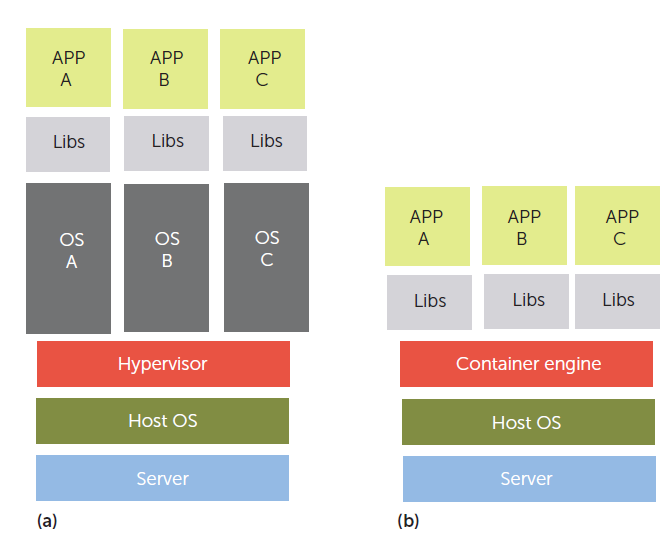
\includegraphics[width=0.7\linewidth]{resources/eea3da004befcc5437960cbc868be634.png}
    \caption{Architectural comparison of (a) virtual machine and (b) container \cite{bernsteinContainersCloudLXC2014}}
    \label{fig:vms-vs-containers}
\end{figure}

\section{Container Orchestration}

As the number of concurrently running containers grows, managing them quickly becomes challenging. Therefore, some form of automation is required to ease this orchestration process at scale. This is precisely the issue that \textit{container orchestration} (CO) tools aim to solve. Similar to an orchestra conductor, CO technologies ensure that distributed containers work together harmoniously. By employing OC frameworks, enterprises and organisations can improve how resources are allocated, as well as simplify how they manage containers in cloud-native settings \cite{truyenComprehensiveFeatureComparison2019}.

CO frameworks such as Kubernetes and Docker Swarm effectively manage the deployment, scaling, and networking of containers across multiple machines, allowing the machines to form clusters of interconnected computers that act as unified computing units. These units can then handle containerised workloads, offloading the management responsibilities (connectivity, workload scheduling, scaling, resource allocation, etc.) from application developers \cite{Nodes, UsingMinikubeCreate}. In other words, from the developer's perspective, the cluster can be treated as a single computing unit to schedule workloads to. This configuration allows containerised applications to be distributed across multiple nodes in a straightforward manner. The design pattern, known as \textit{distributed application}, is one of the most common design patterns in cloud computing due to its scalability and resiliency \cite{fehling2014cloud,kratzkeUnderstandingCloudnativeApplications2017}.

CO platforms complement these benefits of distributed and containerised applications by minimising the management overhead and reducing the complexity of maintaining such configuration. The importance of workload distribution and containerisation in cloud infrastructure combined with the added benefits of CO platforms make them an important topic for research in both academia and industry. In 2017, Kratzke et al. \cite{kratzkeUnderstandingCloudnativeApplications2017} found that CO platforms and cloud-native application principles were the research topics that gathered the most attention in the cloud-native space. Cloud-native technologies have evolved significantly since 2017. However, CO platforms still play a central role in today's cloud. The prevalence of CO platforms can be seen from the popularity of Kubernetes as a project, which is discussed in Section \ref{kubernetes}


\section{Cloud-native}
There are a variety of components that constitute the cloud-native design paradigm. As proposed by Gannon et al. \cite{gannonCloudNativeApplications2017}, cloud-native applications are designed to take advantage of the cloud environment. This entails utilising the fluid and distributed nature of the cloud to provide services that can operate at a global scale with low latency and high reliability \cite{gannonCloudNativeApplications2017}.

The Cloud Native Computing Foundation (CNCF), part of the Linux Foundation, seeks to drive forward the cloud-native technologies and practices. They are the leading body in terms of setting recommendations for best practices in the cloud-native space. Many of the projects that they support, such as Kubernetes, Prometheus, HELM, and Argo CD become de facto tools for cloud-native application development, monitoring, orchestration, and deployment. CNCF defined cloud-native technologies as those that enable the development and deployment of scalable applications in cloud environments \cite{cloudnativecomputingfoundationWhoWeAre}. The application could be hosted on a public, private, or hybrid cloud. However, to support the above-mentioned requirements for latency, reliability, and scalability, they usually possess the following attributes:

\begin{enumerate}
\item
  \textbf{Containers}: Compact, self-sufficient units containing all the necessary components to run software, promoting uniformity from development through to deployment.
\item
  \textbf{Service Meshes}: Infrastructure layer that facilitates direct and manageable communication within microservices setups, enhancing clarity and control over service interactions.
\item
  \textbf{Microservices}: Design philosophy that organises applications into a network of small, independent services, each fulfilling a specific atomic function.
\item
  \textbf{Immutable Infrastructure}: A method that involves renewing or reconstructing infrastructure elements instead of modifying them, aiming to minimise discrepancies and prevent failures.
\item
  \textbf{Declarative APIs}: Interfaces that enable developers to define their requirements explicitly without detailing the execution process, streamlining application oversight by hiding the complexity of the underlying operations.
\end{enumerate}

\section{Kubernetes}\label{kubernetes}
\subsection{Background}

Developed by Google and later donated to the CNCF, Kubernetes (K8s) is an open-source CO platform for automating the deployment, scaling, and operation of application containers \cite{Kubernetes}. Currently, it is one of the most popular cloud-native technologies with over 111,000 stars on GitHub, and it has been accepted as the industry standard for container orchestration \cite{truyenComprehensiveFeatureComparison2019, KubernetesKubernetesProductionGrade}. It is specifically built to scale and is capable of orchestrating thousands of containers across multiple environments (public, private, and hybrid clouds).

Kubernetes offers several key features that make it well-suited for cloud-native application management:

\begin{itemize}

\item \textbf{Automated Scheduling}: Container placement in a cluster is done by automatically scheduling workloads considering resource availability and constraints to maximise infrastructure efficiency. 

\item \textbf{Self-Healing}: Kubernetes monitors the health of containers and nodes in the cluster and attempts to recover them in case of failures by initiating restart or rescheduling tasks.

\item \textbf{Horizontal Scaling}: Applications can adjust the number of container instances based on real-time demand automatically or manually in response to specified metric(s).

\item \textbf{Service discovery and load balancing}: Service discovery is simplified via the use of DNS names or IP addresses, evenly distributing network traffic among containers.

\item \textbf{Storage Orchestration}: Containers can have storage set up that is handled automatically with a wide variety of options including local storage, cloud-provisioned storage, and network file systems.

\item \textbf{Secret and Configuration Management}: Kubernetes handles sensitive data such as passwords, tokens, and configuration details and ensures that only the designated containers have access to them. 

\end{itemize}

In addition to its core functionality, Kubernetes has fostered a diverse portfolio of supportive tools and services such as Helm for package management, Prometheus for monitoring purposes, and ArgoCD for continuous delivery \cite{Helm, prometheusOverviewPrometheus, ArgoCDDeclarative}. This ecosystem plays a significant role in solidifying Kubernetes' central position in the modern cloud-native landscape.

\subsection{Distributions}
As a widely adopted tool across various industries, it is challenging for the upstream Kubernetes distribution to cater to all the requirements and use cases of its users. Thus, different Kubernetes \textit{distributions} emerged to address these specific needs, such as lightweight deployment and managed deployment \cite{bohmProfilingLightweightContainer2021, pereiraferreiraPerformanceEvaluationContainers2019}. From the licensing and management perspective, Kubernetes distributions largely fall into two categories: open-source (self-managed) and proprietary (managed).

\subsubsection{Open-source Kubernetes Distributions}

For organisations that prioritise flexibility, one option is to adopt an open-source Kubernetes distribution. Due to the lack of standards, there are certain differences between cloud service providers. According to Truyen et al. \cite{truyenManagingFeatureCompatibility2020}, these discrepancies largely fall into the following groups: cluster architecture and setup; framework customisation interfaces; and feature incompatibilities. Disparities between vendors can create compatibility challenges when the need for platform migration arises. Open-source solutions' main strength is mitigating the risk of vendor lock-in \cite{shaikh2011total}. The differences will be discussed in further detail in the Related Works section.

\subsubsection{Managed Kubernetes Distributions}

Despite the high degree of customisability and flexibility that open-source solutions offer, they lack the advanced features that managed Kubernetes distributions offer. These features could include, for instance, automated control plane management (updating and maintaining Kubernetes control plane); cluster auto-scaling (scaling the underlying collection of compute nodes according to demand); and Kubelet configuration APIs (the underlying Kubernetes process on each node can be configured through APIs instead of command-line parameters) \cite{truyenManagingFeatureCompatibility2020, KubeletConfigMachineconfigurationopenshiftioV1, AmazonEKSCustomers, RedHatOpenShiftb}. As a result, there is a significant disparity in adoption, with organisations favouring managed solutions over open-source ones \cite{redhatinc.StateKubernetesSecurity2024}.

\paragraph{Managed Kubernetes in the Cloud}\label{par:managed-kubernetes}\mbox{}

In the context of managed Kubernetes, some major public cloud options are Amazon Elastic Kubernetes Service (EKS), Google Kubernetes Engine (GKE), Azure Kubernetes Service (AKS), Red Hat OpenShift \footnote{At the time of writing, OpenShift offer five public cloud provider options for cloud-hosted infrastructure: AWS, Azure, Google, and IBM \cite{OpenShiftContainerPlatform}}, and VMware Tanzu \cite{AmazonEKSCustomers, nickomangAzureKubernetesService, GKEOverviewGoogle, redhatinc.RedHatOpenShift, VMwareTanzuPlatform}.

This thesis focuses strictly on managed Kubernetes offerings in the public cloud, due to the limited availability of pricing information for the self-managed/private cloud option. For instance, Red Hat OpenShift pricing information for the public cloud editions is accessible through their website \cite{redhatinc.RedHatOpenShift}. However, the self-managed version requires contact with a sale person \cite{RedHatOpenShifte}. In addition, as mentioned in Section \ref{subsec:public-cloud}, it is the most common cloud deployment model. Pereira et al. \cite{pereiraferreiraPerformanceEvaluationContainers2019} suggested that this is true for Kubernetes hosting preference as well, with cloud-hosted Kubernetes becoming more common. In the paper, this was attributed to the auto-provisioning (or auto-scaling) capability, along with the management aid that cloud-hosted Kubernetes offers.

\section{Interest in Kubernetes and Managed Kubernetes}

\subsection{Google Trends}

\FloatBarrier  

\begin{figure}
    \centering
    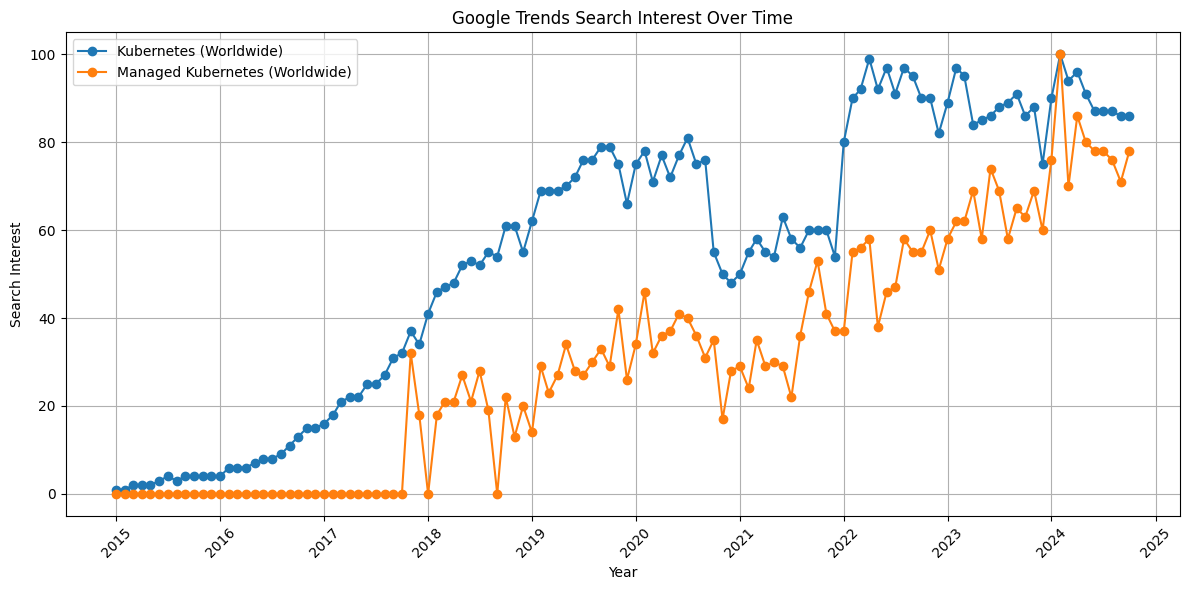
\includegraphics[width=1\linewidth]{resources/d2a89eeeda76d50039bc6f5d3a97c41b.png}
    \caption{Google Trends search interest in Kubernetes vs managed Kubernetes}
    \label{fig:search-interests-kubernetes-vs-managed-kubernetes}
\end{figure}

To provide context for the topic covered in this thesis, this section looks at the popularity of Kubernetes and managed Kubernetes by examining Google Trends search data and the yearly publications data from the Web of Science database. Kratzke et al. proposed that Google Trends can serve as a resource for spotting “industrial buzzwords” and new trends in the technology sector \cite{kratzkeUnderstandingCloudnativeApplications2017}. By combining this data with an analysis of research publications, we can gain insights into evolving trends in both industry and academia. The keywords examined are “Kubernetes” and “managed Kubernetes” (case-insensitive). The timeframe spans from the earliest data point in 2015 to October 2024, which is one month prior to the completion of this thesis.

Figure \ref{fig:search-interests-kubernetes-vs-managed-kubernetes} shows the search interest on Google for “Kubernetes” compared to “managed Kubernetes”. From this graph, it can be discerned that there has been a steady rise in popularity for Kubernetes since its introduction until the peak around 2022, after which the search interest stabilises.

One noteworthy aspect is the decline in search activity observed in 2021; however, the reason behind this decline remains ambiguous. Similar search trends were observed for various cloud-native technologies such as Docker and Fluentd, showing comparable decreases. This commonality suggests that although the root cause remains unknown, this change may have influenced a wide array of adjacent technologies in the cloud-native sphere.

The Google Trends data highlights a convergence in interest for Kubernetes and managed Kubernetes, especially in recent years. The growing preference for managed Kubernetes could indicate a rising awareness among users and businesses about the benefits of managed solutions.

The preference for managed Kubernetes is further supported through industrial reports and surveys. For instance, a 2022 report by Canonical indicated that only 19.3\% of respondents use native (self-managed) Kubernetes \cite{canonicalKubernetesCloudNative2022}. Similarly, Red Hat's 2024 state of Kubernetes security report showed comparable data, with just 23\% of respondents using self-managed Kubernetes \cite{redhatinc.StateKubernetesSecurity2024}.

\subsection{Research Publications}\label{subsec:research-publications}

\FloatBarrier

\begin{figure}
    \centering
    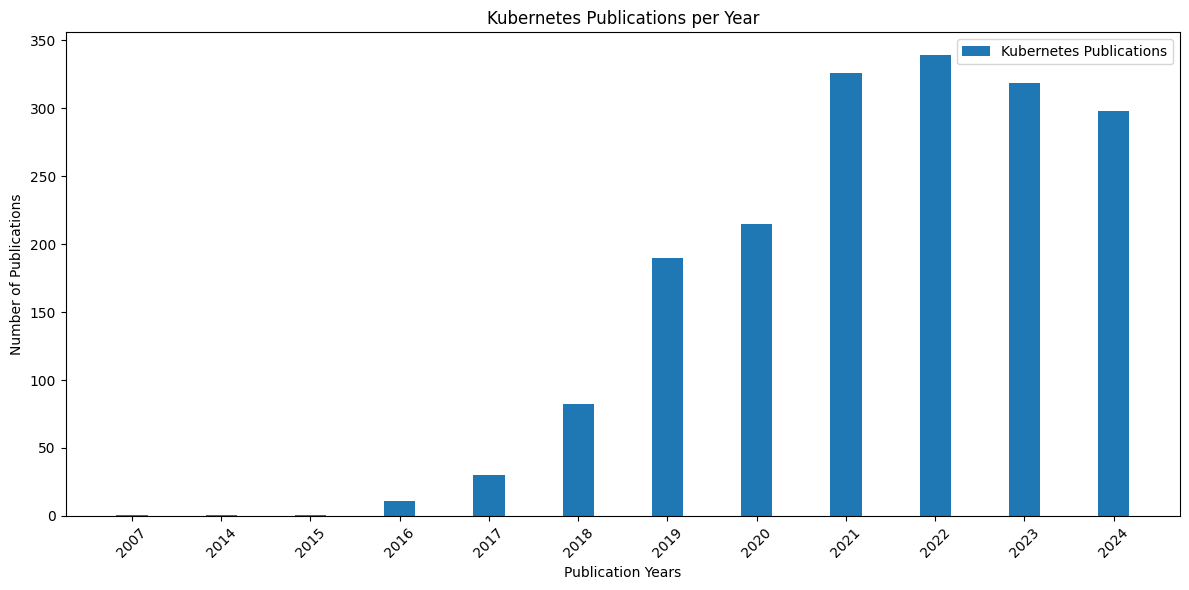
\includegraphics[width=1\linewidth]{resources/publications-plot-k8s.png}
    \caption{Annual research publications on Kubernetes}
    \label{fig:research-publications-kubernetes-and-managed-kubernetes}
\end{figure}


\begin{figure}
    \centering
    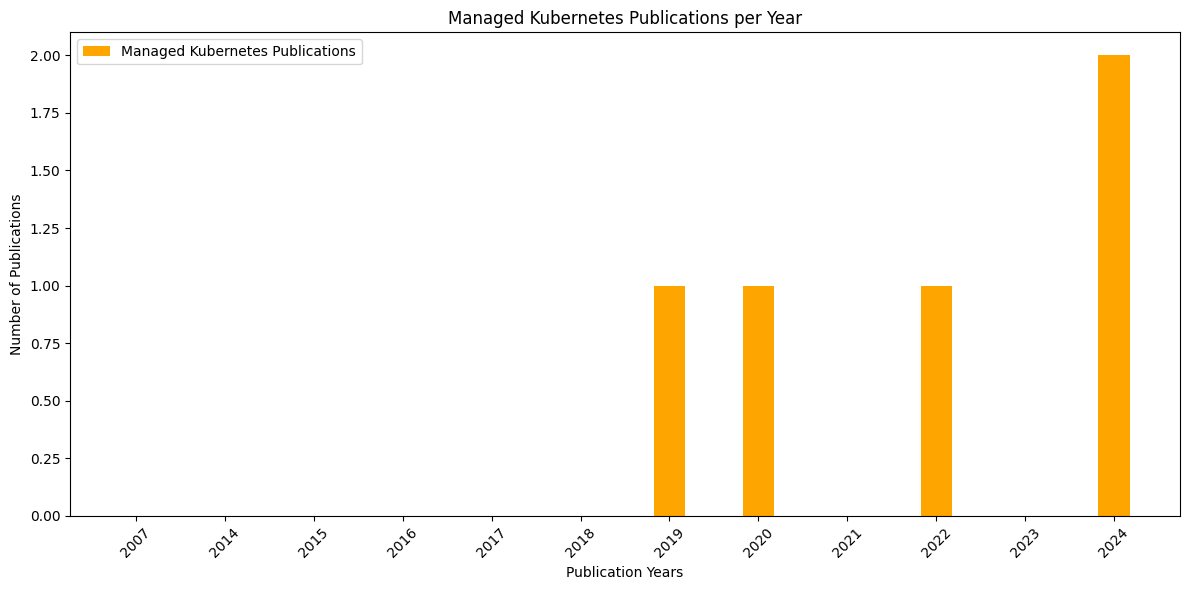
\includegraphics[width=1\linewidth]{resources/publications-plot-managed-k8s.png}
    \caption{Annual research publications on managed Kubernetes}
    \label{fig:research-publications-managed-kubernetes}
\end{figure}

This process of analysing academic interest in the given topics involved collecting information on the yearly publication count through the Web of Science result analysis tool. The annual publication data, shown in Figure \ref{fig:research-publications-kubernetes-and-managed-kubernetes}, reflects a steady increase in Kubernetes-related publications until the peak in 2022. This trend aligns with the results demonstrated by the Google Trends data.

The term ``managed Kubernetes'' was chosen because it appears to be a common term for distributions such as AKS, EKS, GKE, and OCP \cite{AmazonEKSCustomers,ManagedKubernetesService,pereiraferreiraPerformanceEvaluationContainers2019}. However, as depicted in Figure \ref{fig:research-publications-managed-kubernetes}, the number of hits for ``managed Kubernetes'' was surprisingly low. To widen the scope of the search, the following query was used to capture all mentions of these distributions in the topic: \texttt{`TS=((EKS OR "Elastic Kubernetes Service" OR AKS OR "Azure Kubernetes Service" OR GKE OR "Google Kubernetes Engine" OR OCP OR "OpenShift Container Platform" OR "managed kubernetes") AND "kubernetes")`}. This query matches all results with any of the managed Kubernetes distributions mentioned in the title, abstract, or keywords. In addition, it filters out any results that \textit{do not} contain the word ``Kubernetes''. This aims to avoid irrelevant matches from other fields (for example, medicine and biology) that are unrelated to the current search.

Plotting the results again, it can be observed that although the number of matches (Figure \ref{fig:managed-k8s-broaden-scope}) has increased compared to the previous query with \texttt{``managed kubernetes''}. However, the number of publications remains at a modest amount from 2019 to 2023. Although, there was a spike in the number of publications in 2024. It is unclear whether this is a temporary increase or the start of a long-term trend in managed Kubernetes research.

\FloatBarrier


\begin{figure}
    \centering
    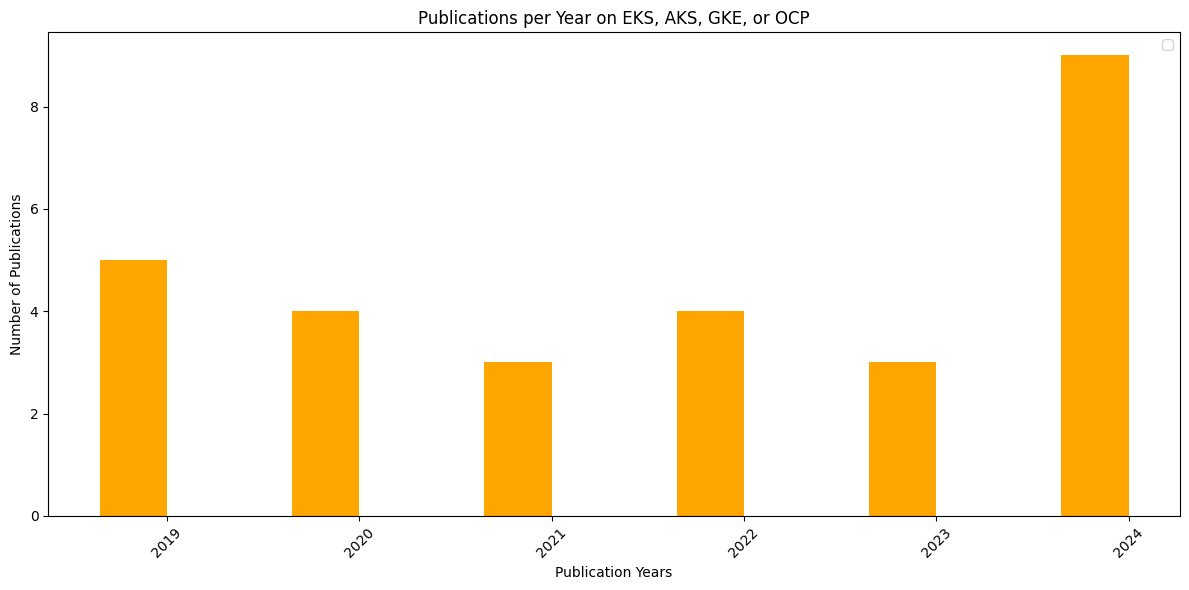
\includegraphics[width=1\linewidth]{resources/managed-k8s-broaden-scope.png}
    \caption{Annual research publications on the managed Kubernetes distributions examined (EKS, AKS, GKE, OCP)}
    \label{fig:managed-k8s-broaden-scope}
\end{figure}


Nevertheless, it is worth noting that managed Kubernetes has not received the same level of attention in academic research as it has in Google Trends. There was only a rather limited number of publications about it annually from 2019 to 2024. As observed by Bunse et al. \cite{BUNSE2011667}, there are potential research gaps between what the industry needs and what has been researched in the available scientific literature. Given the available data, it is possible that despite growing interests, ``managed Kubernetes'' has not received adequate research attention. This disparity indicates that there is potential for further academic investigation into managed Kubernetes (e.g. features, performance, and costs), similar to the work from Ferreira et al. \cite{pereiraferreiraPerformanceEvaluationContainers2019}.

Regarding the observed peak in publications on ``Kubernetes'', a 2019 study by Truyen et al. \cite{truyenComprehensiveFeatureComparison2019} proposed that container orchestration technologies were entering the peak of the Gartner hype cycle. However, both the Google Trends data and the number of annually published articles seem to suggest otherwise. From these insights, it appears that Kubernetes likely reached its peak in popularity in 2022.

These statistics indicate a rising interest in both Kubernetes and managed Kubernetes, highlighting the relevance of the thesis topic. The increasing interest in managed Kubernetes, combined with the lack of research evaluating managed Kubernetes solutions, demonstrated a potential for further academic exploration and analysis to address this gap. With the focus on examining the most suitable managed Kubernetes distribution, the thesis falls under the ``best of breed'' stream of research. It was mentioned by Marston et al. \cite{MARSTON2011176} that this research stream is a highly relevant vein of research for cloud computing.

\section{Academic Literature on Managed Kuberentes Distributions Evaluation}

As mentioned by Pereira et al. \cite{pereiraferreiraPerformanceEvaluationContainers2019}, as well as demonstrated by the number of yearly publications in section \ref{subsec:research-publications}, the literature covering the performance of managed solutions is rather sparse. Open-source Kubernetes distributions, on the other hand, have received significantly more attention in terms of research \cite{bohmProfilingLightweightContainer2021,koziolekLightweightKubernetesDistributions2023,ascensaoAssessingKubernetesDistributions2024,9660392,bryantKubernetesDeploymentOptions2024}. Given the degree of variations amongst the managed distributions in terms of performance, features, and costs, further research could provide valuable insights that aid organisations in making informed decisions on their distribution of choice.

Nevertheless, a selection of relevant literature was identified from the search query in section \ref{subsec:research-publications}. This section provides discussions on these works and relates them to the current thesis.

\subsubsection{Differences Between Kubernetes Vendors and Vendor Lock-in}
Truyen et al. \cite{truyenManagingFeatureCompatibility2020} looked at three major Kubernetes distributions (EKS, AKS, GKE) and compared them in terms of feature compatibility and the potential for vendor lock-in. The main groups of differences proposed are:

\begin{itemize}

\item \textbf{Architectural}: Differences in terms of the way the platform is implemented. For example, the operating system choice of the platform.
\item \textbf{Customization interfaces}: Differences in terms of how Kubernetes components can be configured. For example, the Container Network Interface (CNI) choices that the distribution provides (Calico, Cilium, Flannel, etc.)
\item \textbf{Feature incompatibilities}: Differences in terms of feature availability. This could be in the form of API resources, Custom Resource Definitions (CRDs), etc. For example, the Vertical Pod Autoscaler add-on is a CRD that is only supported in GKE.

\end{itemize}

These divergences can bring migration challenges, which introduces a risk called \textit{vendor lock-in}. Vendor lock-in happens when an organisation becomes dependent on a product and alternative options require significant efforts (e.g. costs, technical, legal) \cite{opara2016critical}.



\subsubsection{Ease of Migration Analysis}

Due to the mentioned differences between platforms, migrating from one platform to another can prove to be a challenging procedure. Truyen et al. \cite{truyenManagingFeatureCompatibility2020} evaluated AKS, EKS, and GKE in terms of pair-wise migratability mapping across these differences \cite{truyenManagingFeatureCompatibility2020}. 

The paper discussed potential errors in the recorded test output due to some test results being inconsistent with the official documentation. In these tests, the feature in question is supported according to the documentation, despite the test results suggesting otherwise. After adjusting for the errors (i.e., using the documentation's status as a reference), EKS possesses the lowest number of incompatible occurrences, making it the most configurable distribution out of the ones examined. In other words, when strictly considering their compatibility with native Kubernetes' customisation interfaces, EKS is more compatible than the other two vendors \textit{after potential configurations}.

GKE, on the other hand, has the highest number of Kubernetes features that work \textit{out-of-the-box}. This means that with zero configurations, GKE is the most compatible with native Kubernetes' feature set and is the most feature-rich distribution.

The work shows that there are non-negligible differences even among major players in the managed Kubernetes space and the compatibility between evaluated platforms. However, the paper did not assess the importance of the features provided by the platforms as well as the differences in the cost of operation. In addition, OCP was not evaluated in the study. As one of the most popular managed Kubernetes distributions, there are potentially valuable insights that can be obtained from examining OCP and comparing it against other offerings \cite{redhatinc.StateKubernetesSecurity2024, vrabicDigitalTwinsUnderstanding2018, portworxKubernetesAdoptionSurvey2021, broadcomStateKubernetes20232023}.


\subsubsection{Performance Analysis of Managed Kubernetes Distributions}

Pereira et al. \cite{pereiraferreiraPerformanceEvaluationContainers2019} evaluated the three major managed Kubernetes distributions (EKS, AKS, and GKE) in terms of performance. The performance was evaluated by four key computing characteristics: CPU, memory, disk, and network. In addition to the selected cloud services, the paper evaluates the performance of the NeCTAR Research Cloud using the same experiment setup to obtain a set of baseline metrics. These metrics from NeCTAR act as a frame of reference to provide further context to how the three services examined perform.

The findings suggested that there is no definitive ``best'' solution that outperforms the others on all metrics examined. However, it was observed that EKS outperform the others on CPU, memory, and disk I/O benchmarks, while GKE possesses superior performance on the network benchmark \cite{pereiraferreiraPerformanceEvaluationContainers2019}.

Similar to \cite{truyenManagingFeatureCompatibility2020}, the paper did not include OCP in the evaluation, and did not include an analysis of feature and costs. However, it was noted that the related costs to the scaling operations of these services could be a potential area to study in the future \cite{pereiraferreiraPerformanceEvaluationContainers2019}.


This thesis focuses on evaluating relevant features for enterprises as identified in Section \ref{evaluation-criteria} in a quantifiable manner. This enables users to perform a multi-criteria appraisal and determine the most appropriate distribution based on their organisation's needs.


\chapter{Evaluation}\label{evaluation-methodology}

This section explains the methodology behind managed Kubernetes service evaluation used in this thesis. The section is structured as follows. Section \ref{sec:multi-criteria-service-selection} discusses potential methods considered, and the reasoning behind the chosen evaluation framework. Followed by Section \ref{evaluation-criteria}, which identifies the relevant features for the current analysis. Then, Section \ref{evaluation-setup} applies the multi-criteria service selection framework to the current research problem and defines the parameters required for the evaluation. Lastly, Sections \ref{result-normalisation} and \ref{result-compilation} discuss the computation and presentation of evaluation results.

\section{Methodology}\label{sec:multi-criteria-service-selection}

The method for evaluating the distributions in this thesis must be
adaptable to qualitative features. In addition, the output of the method
must result in a clear ranking of the evaluated services, making it possible to identify the \textit{most suitable} solution for the user's requirements.

Several methods for cloud service selection were considered for this thesis. The Cloud
Evaluation Experiment Methodology (CEEM) framework used by Pereira
et al.~\cite{pereiraferreiraPerformanceEvaluationContainers2019} in the
managed Kubernetes performance evaluation. However, this framework was designed with empirical experiments
in mind. Thus, it is not applicable to this thesis since most of the
features are qualitative in nature.

Another framework for cloud service selection is proposed by Arun et
al.~\cite{9284492}. It provides a rather comprehensive and structured
method to evaluate cloud services, including a criterion for cloud
features. Yet, the emphasis is on multi-cloud service selection, resulting in a selection of multiple cloud services potentially hosted across different regions. On the contrary, the
current work focuses more on the comparison and ranking between the
services being evaluated as standalone solutions. In other words, a \textit{single cloud} selection problem rather than a multi-cloud one.

Truyen et al. \cite{truyenManagingFeatureCompatibility2020} examined the three managed Kubernetes distributions by performing configuration and e2e testing of k8s features, utilising the testing suite from Kubernetes Special Interest Groups (k8s SIGs). These tests determine whether a given k8s feature is supported by the target vendor or not. Through analysing the test results, the paper quantified the ease of migration of each feature into different levels:


\begin{itemize}
\tightlist
\item
  \textbf{Automated migration:} No additional configuration is needed.
  The k8s feature is supported by the vendor out-of-the-box, or it is
  possible to use the native k8s customisation interface to activate the
  feature.
\item
  \textbf{Uniform reconfiguration:} The feature can be supported on the
  target vendor via performing certain generic reconfigurations using
  the vendor-agnostic Kubernetes API.
\item
  \textbf{Custom translation of input or output data:} The activation of
  the native k8s feature is not supported by the target vendor. However, an
  alternative implementation of the feature is provided that has
  different output or input to the native feature.
\item
  \textbf{Migration is not possible:} The target vendor does not support
  the feature, and there is no alternative feature available.
\end{itemize}

This procedure offers a systematic method to evaluate support for native Kubernetes features on managed Kubernetes distributions. Through the support status of the features, it is possible to evaluate the ease of migration from native Kubernetes to the target distributions. However, since native Kubernetes is the frame of reference, it is unsuitable for evaluating managed Kubernetes distributions against each other in terms of their own feature set (i.e., potential features that native Kubernetes does not have).


One framework
that could potentially match the requirements for the research problem in this thesis is the multi-criteria
selection method suggested by Rehman et al.~\cite{5976164}. The work outlined a formalisation of the multi-criteria service selection problem into mathematical form. Through the framework, a clear suitability ranking of the services can be derived from the user-defined requirements and service performance. This
provides a systematic approach for evaluating the managed Kubernetes distributions.

The key factors involved in the method are:

\begin{enumerate}
\def\labelenumi{\arabic{enumi}.}
\tightlist
\item
  \textbf{Service set (\(S\)):} A set with length \(l\) of all available
  services being evaluated, where element \(s_i\) corresponds to the
  service \(i\).
\item
  \textbf{Performance criteria (\(C\)):} A set with length \(m\) of all
  the criteria being used to evaluate the services in \(S\), where
  element \(c_j\) corresponds to the criteria \(j\).
\item
  \textbf{Performance measurement functions (\(F\)):} A set with length
  \(m\) of functions being used to evaluate the criteria in \(C\). Each
  function \(f_j\) for criterion \(c_j\) can be applied to the service
  \(s_i\) such that \(f_j(s_i)\) results in a quantitative metric as
  output.
\item
  \textbf{Service descriptor (\(D_i\)):} A row vector with length \(m\)
  that contains the evaluations of service \(s_i\), where element
  \(d_j\) of the vector correspond to the result of the performance
  evaluation on criterion \(c_j\) (\(d_j=f_j(s_i)\)).
\item
  \textbf{Decision matrix (\(A\)):} An \(l \times m\) matrix where
  element \(a_{i,j}\) corresponds to the performance of service \(s_i\)
  with regard to criterion \(c_j\). In other words, the row \(a_i\) of
  the matrix is equivalent to the service descriptor vector \(D_i\).
\item
  \textbf{User requirement criteria (\(R\)):} A row vector with length
  \(m\) that contains the user/decision maker's minimum requirements for
  each criterion \(c_j\), where element \(r_j\) is the minimum
  requirement for criterion \(c_j\).
\item
  \textbf{User priority weights (\(W\)):} A row vector with length \(m\)
  that contains the user/decision maker's priority for each criterion
  \(c_j\), where element \(w_j\) is the weight for criterion \(c_j\).
\end{enumerate}

From these factors, we can compute the Exponential Weighted Difference
(EWD):

\[
\begin{pmatrix}
e^{-(a_{1,1} - r_1)w_1} + e^{-(a_{1,2} - r_2)w_2} + \cdots + e^{-(a_{1,m} - r_m)w_m} \\
e^{-(a_{2,1} - r_1)w_1} + e^{-(a_{2,2} - r_2)w_2} + \cdots + e^{-(a_{2,m} - r_m)w_m} \\
\vdots \\
e^{-(a_{l,1} - r_1)w_1} + e^{-(a_{l,2} - r_2)w_2} + \cdots + e^{(a_{l,m} - r_m)w_m} \\
\end{pmatrix}
\]

The calculation results in a column vector of length \(l\), with each
row containing a single number that will be the score of the service
\(s_i\) in our evaluation. This effectively measures how much the
assessment score of a feature deviates negatively from the user's minimum
requirements. A score that is lower than the minimum requirement
\(a_{i,j}<r_j\) would result in a positive power and thus a large
exponential term. On the other hand, a score that is higher than the
minimum requirement would result in a negative power and thus a small
exponential term. A smaller term indicates that the service performs
better than other services in relation to the criteria being evaluated
and the user's requirements.

It can be observed that the formula heavily penalises features that
fall \emph{below} the user's requirements, far more than features that
exceed the user's requirements can compensate (e.g.~\(e^{2} > e^{-2}\)).
In addition, exceeding the minimum requirements is desirable
(e.g.~\(e^{-2}>e^{-3}\)). However, since an exponential function is
used, the gain follows a diminishing return curve as the assessment
score becomes higher. As addressed by Rehman et al.~\cite{5976164}, this
pattern is desirable for two reasons:

\begin{enumerate}
\def\labelenumi{\arabic{enumi}.}
\tightlist
\item
  Ensuring that the user's minimum requirements are respected. In
  practical decision-making, the fact that a service score that is 1 unit lower
  than the minimum requirement on criterion A should not be negated by
  criterion B scoring 1 unit above the minimum requirement.
\item
  Preventing a single criterion from dominating the evaluation results. Due
  to the diminishing return curve, situations where a service excels at a
  single feature, resulting in said service being ranked higher, are
  prevented. In other words, while better performance is rewarded, no
  single criterion can overcompensate for subpar performance on other
  criteria. This ensures a balanced evaluation across all criteria.
\end{enumerate}

As an example, given \(r=3\) and \(w=1\), the exponential term in
question would have the curve in Figure \ref{fig:example-exp-func-graph} as the assessment score \(a\)
varies.

\begin{figure}
    \centering
    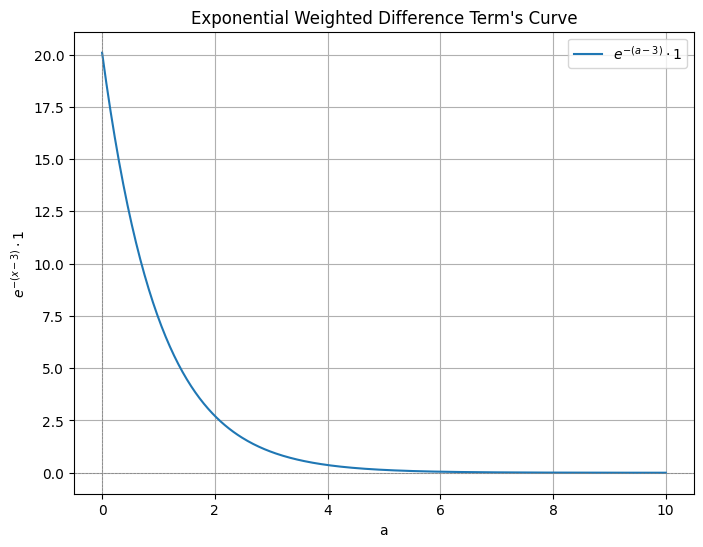
\includegraphics[width=0.75\linewidth]{resources/example exponential function.png}
    \caption{Exponential Weighted Difference term's curve}
    \label{fig:example-exp-func-graph}
\end{figure}

The main challenge for the research problem in this thesis is finding
appropriate functions to evaluate the qualitative features to a numeric
value.

\section{Evaluation Criteria}\label{evaluation-criteria}

This section identifies the relevant criteria for organisations that are evaluated in this thesis. In the chosen multi-criteria selection framework, this corresponds to the criteria set $C$.

For the evaluation, a review of industrial reports was conducted to identify key features for the evaluation. Thereafter, a subset of Kubernetes fundamental features was selected to make the evaluation more realistic and relevant. Lastly, the cost of operation was included, as it is a concern for Nokia as well as other businesses.

\subsection{Key Feature(s)}\label{key-features-for-evaluation}


The goal of this thesis is to investigate suitable managed Kubernetes distributions for enterprises. To achieve this, we must first define what constitutes a “suitable” distribution for enterprise use cases. In other words, the most important factors for companies and organisations when adopting a Kubernetes platform should be identified. Therefore, five major industrial reports from issued between 2022 and 2024 were reviewed. From each report, the three top challenges for adopting Kubernetes or cloud-native platforms are identified.

The five surveys were selected based on the following criteria:

\begin{itemize}
\tightlist
\item
  \textbf{Publication Date:} Between 2022 and 2024 to provide up-to-date insights.
\item
  \textbf{Source:} From large organisations in the cloud space.
\item
  \textbf{Content:} Include insights on various organisational concerns regarding cloud-native development and Kubernetes adoption.
\end{itemize}




There are other related surveys apart from those included in this thesis. However, they did not satisfy one or more of the three criteria defined above. For instance, despite echoing similar sentiments regarding the importance of security in Kubernetes adoption, Red Hat's ``The state of Kubernetes security report: 2024 edition'' report \cite{redhatinc.StateKubernetesSecurity2024} was not included because it focuses heavily on the security aspect, and thus is slightly biased towards security compared to other aspects. Another potential report is Rightscale's ``Cloud computing trends: 2019 state of the cloud survey'' cited by Pereira et al. \cite{pereiraferreiraPerformanceEvaluationContainers2019}. However, this report does not have a more up-to-date version.

The findings from each report are summarised in Table \ref{tab:challenges-from-surveys}.

\begin{tiny} 
\begin{longtable}{|p{0.2\linewidth}|p{0.3\linewidth}|p{0.45\linewidth}|} % Adjusted column widths
\hline
\textbf{Source} & \textbf{Question} & \textbf{Top Challenges} \\
\hline
Portworx 2022 Annual Kubernetes Adoption Report \cite{2022AnnualKubernetes} & What are the challenges that are the most difficult to overcome when running Kubernetes (ranked top three)? & 
\raggedright 1. Security \newline 2. Data management \newline 3. Reliability \tabularnewline
\hline
Broadcom State of Cloud Native App Platforms 2024 Report \cite{StateCloudNative} & What challenges do organizations encounter in building or adopting a cloud native app platform? & 
\raggedright 1. Meeting compliance and security requirements \newline 2. Integration with existing data sources and repositories \newline 3. Distributed ownership deployment and management \tabularnewline
\hline
Canonical Kubernetes and Cloud Native Operations Report 2022 \cite{canonicalKubernetesCloudNative2022} & What are the top challenges Kubernetes brings to businesses? & 
\raggedright 1. Security and compliance concerns not addressed adequately \newline 2. Integrating cloud-native applications together \newline 3. Poor or limited support from platform providers or partners \tabularnewline
\hline
Spectrocloud 2024 State of Production Kubernetes Survey \cite{2024StateProduction} & What challenges does your organization face with running Kubernetes in production? & 
\raggedright 1. It’s difficult to choose and validate the right stack components from the broad cloud-native ecosystem \newline 2. Configuration drift causes issues with compliance and availability \newline 3. We struggle to properly protect ourselves against security breaches \tabularnewline
\hline
CNCF Annual Survey 2023 \cite{CNCFAnnualSurvey2024} & What are your Challenges in Using / Deploying Containers? & 
\raggedright 1. Security \newline 2. Complexity \newline 3. Monitoring \tabularnewline
\hline
\caption{Top challenges for Kubernetes and cloud-native platforms adoption from industrial surveys} \label{tab:challenges-from-surveys} \\
\end{longtable}
\end{tiny}
From these surveys, it is clear that security is the most pressing concern for organisations. Therefore, based on these reports, security is selected as a key indicator of distribution suitability.

It is also evidenced in these reports that other aspects such as complexity of adoption \cite{CNCFAnnualSurvey2024,2024StateProduction}, data management and integration mentioned in \cite{2022AnnualKubernetes,broadcomStateKubernetes20232023} are also important to organisations. However, security is the only feature that appears consistently across all five surveys, indicating that it is undoubtedly a pressing concern for a large portion of organisations surveyed. Thus, to narrow the scope of this thesis, security is the only aspect included in the evaluation. However, given their importance, the complexity and data management aspects could be potential areas for future works to explore.

\subsection{Fundamental Kubernetes Features}

Truyen et al. \cite{truyenManagingFeatureCompatibility2020} suggested that there are differences between distributions apart from security features. Thus, to make the evaluation more realistic, a selection of basic features is included. These are features that directly impact the operation of a Kubernetes cluster, independent of the organisational requirements.

The features selected are:

\begin{enumerate}
  \item \textbf{Storage provisioning:} Number of storage provisioning methods officially supported.
  \item \textbf{CNIs:} Number of CNIs officially supported.
  \item \textbf{Monitoring and logging:} Number of application monitoring and logging methods officially supported.
  \item \textbf{Maximum number of nodes in a cluster:} The node limit for a single cluster.
\end{enumerate}

This thesis limits itself to these criteria. There are other potential features that could be included. However, evaluating them requires separate in-depth experimentation, and therefore they do not fall within the constraints (e.g., budget for hosting managed Kubernetes cluster) of this thesis. For instance, certain features that could be useful to include are the CPU, memory, disk I/O, and networking performance of the distributions. These measurements were examined in further detail by Ferreira et al. \cite{pereiraferreiraPerformanceEvaluationContainers2019}. However, the data from the paper cannot be applied to this thesis since OCP was not included in the analysis.

Despite the limitations, the included features make the current evaluation more multifaceted and relevant to businesses, since they are fundamental features of Kubernetes that directly impact operations.

\subsection{Costs}

An additional issue enterprises consider is cost. For managed Kubernetes, the cost of operation can be further broken down into two main components: management costs and infrastructure costs. Management costs are the fees that service providers charge for managing the Kubernetes cluster(s). Infrastructure costs are charged according to the usage of underlying infrastructure to host the clusters. The total cost of operation from these two components is an important factor that influences enterprises' choice of services. Thus, it is crucial to include the cost of these distributions as a criterion in our evaluation.


\section{Evaluation Setup}\label{evaluation-setup}

Applying the chosen multi-criteria service selection framework to the research problem described in this thesis yields the following parameters and variables for the evaluation setup.

\subsection{Service set and performance
criteria}\label{service-set-and-performance-criteria}

We can define the first two parameters (service set and performance criteria) as follows:

\begin{itemize}
\tightlist
\item
  \textbf{Service set (\(S\)):} (EKS, AKS, GKE, OCP)
\item
  \textbf{Performance criteria (\(C\)):} (Security, Costs, Maximum nodes
  in a cluster, Storage provisioning, CNIs, Monitoring and logging)
\end{itemize}

\subsection{Performance Evaluation
Functions}\label{performance-evaluation-functions}

The performance evaluation functions determine how the score for
each criterion in the criteria set \(C\) is calculated. The functions for each
of the mentioned criteria are defined as follows:

\subsubsection{Security}\label{security}

For all distributions, the security features are examined from a
\emph{functional} perspective. The following question is
evaluated: ``What is the output of this feature?''. Then, the number of features/functions that can be performed is counted.

\subsubsection{Cost}\label{cost}

As mentioned in Section \ref{par:managed-kubernetes}, the costs for public
cloud services are publicly available and are often published on the
provider's website. Therefore, it is possible to estimate the costs of operation on these public clouds through the websites. For all distributions, the following parameters are
used to provide a standardised estimate for the cluster's management
fee:

\begin{itemize}
\tightlist
\item
  \textbf{Region:} Northern Europe (Helsinki is chosen if corresponding hosting options are available. If not, Stockholm is chosen). This makes the
  evaluation more relevant to Nokia and Finnish businesses.
\item
  \textbf{Number of Clusters:} 1
\item
  \textbf{Type of Support/Support License Agreement (SLA):} The most
  extensive option. As stated in the CNCF Annual Survey 2023
  \cite{CNCFAnnualSurvey2024}, complexity is still the second most
  challenging problem for container operations. Thus, an extensive
  degree of support aims to reflect the practical needs of organisations
  when adopting these services.
\end{itemize}

In addition, public cloud services often use the number of vCPUs as the criteria for
management cost calculation
\cite{RedHatOpenShiftc,PricingGoogleKubernetes}. In this evaluation, we
look at a standard cluster with three worker nodes, each with 16 vCPUs. The
full list of VM specifications is as follows:

\begin{itemize}
\tightlist
\item
  16 vCPUs
\item
  64 GB RAM
\item
  1 TB SSD
\item
  Up to 10 Gigabit network bandwidth
\end{itemize}

From these specifications, the monthly costs of operation for EKS, AKS, and GKE are computed
based on the available information on the provider's website. 

For OCP, three public cloud hosting options are available at the time of writing, including Amazon Cloud, Azure Cloud, Google Cloud, and IBM Cloud \cite{RedHatOpenShift}. However, for Amazon and Azure, the infrastructure fee includes the fee for hosting a dedicated control plane with a minimum of 3 master nodes \cite{RedHatOpenShiftc,PricingAzureRed}. This makes the price not comparable to that of the other distributions with managed control planes and pricing scheme based on the number of worker nodes' vCPUs.

Both IBM Cloud and Google Cloud hosting options provide vCPU-based management fee pricing. Of these two, Google Cloud appears to be the more commonly adopted option and therefore was chosen for this evaluation \cite{portworxKubernetesAdoptionSurvey2021}. For the infrastructure fee, as the OpenShift instance is hosted on Google Cloud, it uses the same VM infrastructure. Thus, this option is projected to have the same infrastructure costs as those calculated for GKE, given the same computing specifications.

The total monthly cost of operation is the sum of management and infrastructure costs. Then, the difference between a distribution's monthly cost and the maximum cost of all distributions is calculated. This is conducted to provide a metric that is preferable to maximise. In other words, similar to the other metrics, it is more optimal to have a higher difference from the maximum cost, since that is equivalent to a cheaper offering.

\subsubsection{Maximum Nodes in a Cluster}\label{maximum-nodes-in-a-cluster}

The maximum number of nodes in a cluster is obtained through the
official documentation
\cite{Chapter4Planninga,KnownLimitsService,nickomangLimitsResourcesSKUs2024,QuotasLimitsGoogle}. This limit determines how many nodes can be managed in a given Kubernetes cluster, effectively dictating the maximum scale supported.

\subsubsection{Storage Provisioning, CNIs, and Monitoring/Logging Choices}\label{storage-provisioning-cnis-and-monitoring-and-logging}

For each of these final three criteria, the total number of supported options for the underlying operation is determined from the provider's documentation and used as the evaluation points \cite{WhatAmazonEKS,nickomangAzureKubernetesServicea,GoogleKubernetesEngine,WelcomeOpenShiftContainer}.

\subsection{Minimum Requirements and Weights}\label{performance-evaluation-functions}

The minimum requirement vector $R$ expresses the minimum requirements from the user for each of the criteria evaluated. In the case of costs, the minimum requirement would be the budget of the organisation. For the maximum node limit, the requirement would be the planned number of nodes in the cluster. Similar to the evaluation function output, the user's requirements go through the same normalisation process to obtain values in the same range as the feature scores. As outlined in Section \ref{result-normalisation}, the range chosen in this thesis is 1 to 5.

The weight vector $W$ dictates how important each of the criteria is to the user. Rehman et al. \cite{5976164} did not explicitly specify the range of values for weights. However, as the weights simply scale each term by a factor, the resulting ranking of the services remains the same as long as the weights are proportional. In this thesis, the weights are defined so that they add up to 1. A different range can be selected by simply scaling all weight values by a factor.


\section{Result Normalisation}\label{result-normalisation}

As discussed by Rehman et al.~\cite{5976164}, the performance
measurement functions' results should be normalised to a unified range in order to negate the divergence in result ranges. For example, there are more security features than the number of supported CNIs, resulting in a higher count overall. Thus,
min-max normalisation is performed on all resulting output of the evaluation functions above to
achieve scores on a scale from 1 to 5. The normalisation formula is as follows:

\[
   \text{Normalised Value} = 1 + 4 \times \frac{x - \text{min}(x)}{\text{max}(x) - \text{min}(x)}
\]


\section{Result Compilation}\label{result-compilation}

From all the parameters defined above, it is possible to compute the service
descriptor vector (\(D_i\)) and the decision matrix (\(A\)). Finally,
the decision matrix is transformed into the EWD vector using the formula in section \ref{sec:multi-criteria-service-selection}. This vector
contains the final score of all the distributions evaluated, taking
into account all the mentioned factors. The scores provide insights
into how suitable each distribution is for enterprise use cases based on
the chosen set of parameters.

\chapter{Results}\label{results}

This chapter presents the results for comparing the distributions using the chosen framework. The evaluation results in a service descriptor vector for each criterion. Then, four evaluation scenarios are presented, each with its own set of requirements and weights. With the service descriptor vectors, requirements, and weights, the EWDs are computed and used as indicators of distribution suitability for the examined scenarios.

\section{Security Evaluation}

The security features are identified from the official documentation of the selected services \cite{SecurityComplianceRed,SecurityOverview|,miwithroConceptsSecurityAzure2024,SecurityAmazonEKS}. For each feature, the functional question of ``What is the output of this feature from the user's perspective?'' is evaluated.

Through reviewing the official documentation of the selected vendors, 41 security features were identified and listed in Table \ref{tab:feature_overview} in the Appendix. The table includes a descriptive name of the features, as well as their functional usage. 

From the list of features, the corresponding feature support status is identified in Table \ref{tab:feature_support} in the Appendix.

The number of supported features is aggregated by attributing the following scores to the statuses:


\begin{itemize}
\tightlist
\item
  No: 0
\item
  Partial: 0.5
\item
  Yes: 1
\end{itemize}



The total number of supported features by each distribution and the normalised score can be seen in Table \ref{tab:security-evaluation}.

Observing the table, it appears that the features are fairly comparable in terms of the number of security features supported.

\begin{table}[!ht]
    \centering
    \begin{tabular}{|p{4cm}|p{2cm}|p{2cm}|p{2cm}|p{2cm}|} % Set fixed widths for columns
    \hline
         & EKS & AKS & GKE & OCP \\ \hline
        Distribution Security Feature Count& 30& 33& 35& 33\\ \hline
 Distribution Security Feature Count (Normalised)& 1& 3& 5&3\\\hline
    \end{tabular}
    \caption{Security feature support evaluation results} 
    \label{tab:security-evaluation}
\end{table}

\section{Cost Analysis}

With the computational specifications mentioned in Section \ref{evaluation-setup} and the pricing information from the providers, the following costs are calculated \cite{CreateEstimateConfigure,PricingAzureKubernetes,GoogleCloudPricing,RedHatOpenShiftd}:
\begin{table}[!ht]
    \centering
    \begin{tabular}{|p{4cm}|p{2cm}|p{2cm}|p{2cm}|p{2cm}|} % Set fixed widths for columns
    \hline
         & EKS & AKS & GKE & OCP \\ \hline
        Management Cost & 73 & 72 & 288.03 & 500 \\ \hline
        Infrastructure Cost & 1535.78 & 1867.06 & 2541.97 & 2541.97 \\ \hline
        Total Cost & 1608.78 & 1939.06 & 2830 & 3041.97 \\ \hline
        Maximum Cost Difference & 1433.19 & 1102.91 & 211.97 & 0 \\ \hline
        Maximum Cost Differences (Normalised) & 5 & 4.078 & 1.592 & 1 \\ \hline
    \end{tabular}
    \caption{Costs evaluation results} 
    \label{tab:cost-analysis}
\end{table}


\FloatBarrier

The total cost can be broken down further into the management cost and the infrastructure cost. Management cost is the sum providers charge for managing the Kubernetes cluster. This is usually calculated based on the total number of vCPUs a cluster has.

The infrastructure cost denotes the cost of the underlying virtual machines used for the cluster. In this evaluation, it is the cost for the three virtual machines with pre-defined specifications in Section \ref{cost}.

The difference from the maximum cost is also calculated. A higher difference from the maximum cost indicates a service with a lower price.

\section{Fundamental Features Evaluation}

From the documentation, the followings were identified:

\textbf{Maximum Nodes per Cluster}

\begin{itemize}
\tightlist
\item
  EKS: 5,000 \cite{KnownLimitsService}
\item
  AKS: 5,000  \cite{nickomangLimitsResourcesSKUs2024}
\item
  GKE: 5,000 \cite{QuotasLimitsGoogle}
\item
  OCP: 2,000  \cite{Chapter4Planning}
\end{itemize}

The maximum node limits can be found in the official documentation for AKS, EKS, and OCP. In the case of
GKE, while it is theoretically possible to increase the limit to 65,000
nodes, this requires special conditions and configurations. In addition,
special arrangements with GKE support are also required. Thus, the 5,000-node limit is used instead. This is also the limit that was used by
Truyen et al.~\cite{truyenManagingFeatureCompatibility2020}.

\textbf{Storage:}

\begin{itemize}
\tightlist
\item
  EKS: 4 options supported
  S3 \cite{StoreApplicationData}
\item
     AKS: 6 options supported \cite{tamramConceptsStorageAzure2024}
\item
  GKE: 8 options supported \cite{StorageGKEClusters} 
\item
  OCP: 13 options supported \cite{UnderstandingPersistentStorage} 
\end{itemize}

\textbf{CNIs:}

\begin{itemize}
\tightlist
\item
  EKS: 5 CNIs supported \cite{AlternateCNIPlugins}
\item
  AKS: 4 CNIs supported \cite{schaffererinConceptsCNINetworking2024}
\item
  GKE: 4 CNIs supported \cite{NetworkOverviewGooglea}
\item
  OCP: 6 CNIs supported \cite{CertifiedOpenShiftCNI2024}
\end{itemize}

\textbf{Application Monitoring and Logging:}

\begin{itemize}
\tightlist
\item
  EKS: 1 option, Amazon Cloud Watch \cite{MonitorYourCluster}
\item
  AKS: 1 option, Azure Monitor \cite{martinekuanMonitorMicroservicesApplication}
\item
  GKE: 1 option, GKE logging agent \cite{GKELogsGoogle} 
\item
  OCP: 1 option, Loki Stack \cite{Logging60Logging}
\end{itemize}

The supported features and the normalised score for this section are given in Table \ref{tab:fundamental-features-scores}:

\begin{table}[!ht]
    \centering
    \begin{tabular}{|p{4cm}|p{2cm}|p{2cm}|p{2cm}|p{2cm}|} % Set fixed widths for columns
    \hline
         & EKS & AKS & GKE & OCP \\ \hline
        Supported Storage Provisioning Options & 4& 6& 8& 13\\ \hline
        Supported Storage Provisioning Options (Normalised)& 1& 1.89& 2.78& 5\\ \hline
        Supported CNI Options& 5& 4& 4& 6\\ \hline
        Supported CNI Options (Normalised)& 3& 1& 1& 5\\ \hline
        Supported Logging Options& 1& 1& 1& 1\\ \hline
 Supported Logging Options (Normalised)\tablefootnote{All distributions support the same number of application logging options. Thus, the usual min-max normalisation can not be applied due to the dividing by zero error. As long as they all have the same values, this logging criterion should not impact the final evaluation results. For this evaluation, 0 is selected as the logging evaluation score for all distributions.}& 0& 0& 0&0\\\hline
 Maximum Nodes& 5000& 5000& 5000&2000\\\hline
 Maximum Nodes (Normalised)& 5& 5& 5&1\\\hline
    \end{tabular}
    \caption{Fundamental features evaluation results} 
    \label{tab:fundamental-features-scores}
\end{table}

\FloatBarrier

\section{EWD}


All the normalised scores computed are compiled in table \ref{tab:normalised-scores}. 

\begin{table}[!ht]
    \centering
    \begin{tabular}{|p{4cm}|p{2cm}|p{2cm}|p{2cm}|p{2cm}|} % Set fixed widths for columns
    \hline
         & EKS& AKS& GKE& OCP\\ \hline
        Normalised Security& 1.00& 3.00& 5.00& 3.00\\ \hline
        Normalised Cost& 5.00& 4.08& 1.59& 1.00\\ \hline
        Normalised Max Nodes& 5.00& 5.00& 5.00& 1.00\\ \hline
        Normalised Storage& 1.00& 1.89& 2.78& 5.00\\ \hline
        Normalised CNI& 3.00& 1.00& 1.00& 5.00\\ \hline
 Normalised Logging& 0.00& 0.00& 0.00&0.00\\\hline
    \end{tabular}
    \caption{Normalised feature scores} 
    \label{tab:normalised-scores}
\end{table}

Based on the normalised scores, it is possible to calculate the EWD according to the user's requirements and feature weights, which are expressed in the multi-criteria selection framework as the minimum requirement vector ($R$) and the weight vector ($W$). This section presents the calculation performed on a selection of hypothetical scenarios to provide insights to how the suitability of each distribution changes according to specific organisational needs.

Based on the ranges of the feature evaluation scores (1 to 5), minimum requirements (1 to 5), and weights (0 to 1), the exponential term $e^{-(a_{i,j} - r_j)w_j }$ of feature $j$ for service $i$ has the range $\left[e^{-4}, e^{4}\right]\approx \left[0.018,54.598\right]$. However, this range is calculated with a weight of 1, as that is the maximum weight value possible. Since all the weights add up to 1, the range for $e^{-(a_{i,j} - r_j)w_j }$ is much narrower in practice. For instance, with a weight of 0.2, the range of the exponential term is $\approx\left[0.449,2.225\right]$. As discussed in section \ref{sec:multi-criteria-service-selection}, a smaller EWD value indicates higher suitability for the scenario, while a large value indicates that the distribution deviates negatively from the user requirements (i.e., failure to meet the requirements).


\subsection{Scenario 1: Security Prioritisation}

Based on the surveys in section \ref{key-features-for-evaluation}, security is evidently the most important feature for enterprises. To reflect this, security is given a weight of 0.5, while the other features share the other half of the weight and receive equal weights of 0.1 each. As for minimum requirements, since this evaluation does not cater to any single organisation, the requirements are set at 0. The parameters are as follows:

\begin{enumerate}
\def\labelenumi{\arabic{enumi}.}
\tightlist
\item
  \textbf{User requirement criteria (\(R\)):} 0
\item
  \textbf{User priority weights (\(W\)):}

  \begin{itemize}
  \tightlist
  \item
    \textbf{Security:} 0.5
  \item
    \textbf{Costs:} 0.1
  \item
    \textbf{Maximum nodes:} 0.1
  \item
    \textbf{Storage provisioning:} 0.1
  \item
    \textbf{CNIs:} 0.1
  \item
    \textbf{Monitoring and logging:} 0.1
  \end{itemize}
\end{enumerate}

Using the normalised scores obtained through the evaluation functions and the parameters above, the following exponential terms and EWDs can be computed.

\begin{table}[!ht]
    \centering
    \begin{tabular}{|p{4cm}|p{2cm}|p{2cm}|p{2cm}|p{2cm}|} % Set fixed widths for columns
    \hline
 & EKS& AKS& GKE& OCP\\ \hline
        Exp Security & 0.61 & 0.22 & 0.08 & 0.22 \\ \hline
        Exp Cost & 0.61 & 0.67 & 0.85 & 0.90 \\ \hline
        Exp Max Nodes & 0.61 & 0.61 & 0.61 & 0.90 \\ \hline
        Exp Storage & 0.90 & 0.83 & 0.76 & 0.61 \\ \hline
        Exp CNI & 0.74 & 0.90 & 0.90 & 0.61 \\ \hline
        Exp Logging & 1.00 & 1.00 & 1.00 & 1.00 \\ \hline
 EWDs& 4.47& 4.23& 4.20&4.25\\\hline
    \end{tabular}
    \caption{Scenario 1: Exponential Weighted Difference results} 
    \label{tab:scenario-1-ewds}
\end{table}

Lower EWDs indicate higher suitability for the user-defined parameters. Therefore, in this scenario with security being the top priority, GKE appears to be the most suitable distribution.

\subsection{Scenario 2: Costs Prioritisation}

In this scenario, the cost of operation is prioritised. Thus, a weight of 0.5 is assigned to cost, while other features share weights of 0.1. In addition, a monthly budget constraint of 3,000 USD is also introduced. After applying the same normalisation steps to this budget, the following parameters are used:

\begin{enumerate}
\def\labelenumi{\arabic{enumi}.}
\tightlist
\item
  \textbf{User requirement criteria (\(R\)):}
    \begin{itemize}
  \tightlist
  \item
    \textbf{Security:} 0
  \item
    \textbf{Costs:} 3.9
  \item
    \textbf{Maximum nodes:} 0
  \item
    \textbf{Storage provisioning:} 0
  \item
    \textbf{CNIs:} 0
  \item
    \textbf{Monitoring and logging:} 0
  \end{itemize}
\item
  \textbf{User priority weights (\(W\)):}

  \begin{itemize}
  \tightlist
  \item
    \textbf{Security:} 0.1
  \item
    \textbf{Costs:} 0.5
  \item
    \textbf{Maximum nodes:} 0.1
  \item
    \textbf{Storage provisioning:} 0.1
  \item
    \textbf{CNIs:} 0.1
  \item
    \textbf{Monitoring and logging:} 0.1
  \end{itemize}
\end{enumerate}

These parameters result in the following EWDs:

\begin{table}[!ht]
    \centering
    \begin{tabular}{|p{4cm}|p{2cm}|p{2cm}|p{2cm}|p{2cm}|} % Set fixed widths for columns
    \hline
         & EKS& AKS& GKE& OCP\\ \hline
        Exp Security & 0.90 & 0.74 & 0.61 & 0.74 \\ \hline
        Exp Cost & 0.58 & 0.92 & 3.18 & 4.28 \\ \hline
        Exp Max Nodes & 0.61 & 0.61 & 0.61 & 0.90 \\ \hline
        Exp Storage & 0.90 & 0.83 & 0.76 & 0.61 \\ \hline
        Exp CNI & 0.74 & 0.90 & 0.90 & 0.61 \\ \hline
        Exp Logging & 1.00 & 1.00 & 1.00 & 1.00 \\ \hline

 EWDs& 4.74& 5.00& 7.06 & 8.14\\\hline
    \end{tabular}
    \caption{Scenario 2: Exponential Weighted Difference Results} 
    \label{tab:scenario-2-ewds}
\end{table}

It can be observed that the rankings have changed as compared to Scenario 1. Due to the high costs, OCP is now at the bottom of the ranking. On the contrary, thanks to possessing the lowest costs, EKS was elevated to the top, making it the most suitable distribution in this cost-saving scenario.

\subsection{Scenario 3: Maximum Node Requirements}\label{subsec:evaluation-scenario-3}

In this scenario, the organisation is assumed to require at least 3,000 nodes for their Kubernetes cluster. All parameters are the same as that of Scenario 1, except the maximum node now has a minimum requirement of 3,000. After normalisation, the following parameters were chosen:

\begin{enumerate}
\def\labelenumi{\arabic{enumi}.}
\tightlist
\item
  \textbf{User requirement criteria (\(R\)):}
    \begin{itemize}
  \tightlist
  \item
    \textbf{Security:} 0
  \item
    \textbf{Costs:} 0
  \item
    \textbf{Maximum nodes:} 2.33
  \item
    \textbf{Storage provisioning:} 0
  \item
    \textbf{CNIs:} 0
  \item
    \textbf{Monitoring and logging:} 0
  \end{itemize}
\item
  \textbf{User priority weights (\(W\)):}

  \begin{itemize}
  \tightlist
  \item
    \textbf{Security:} 0.5
  \item
    \textbf{Costs:} 0.1
  \item
    \textbf{Maximum nodes:} 0.1
  \item
    \textbf{Storage provisioning:} 0.1
  \item
    \textbf{CNIs:} 0.1
  \item
    \textbf{Monitoring and logging:} 0.1
  \end{itemize}
\end{enumerate}

These parameters result in the following EWDs:

\begin{table}[!ht]
    \centering
    \begin{tabular}{|p{4cm}|p{2cm}|p{2cm}|p{2cm}|p{2cm}|} % Set fixed widths for columns
    \hline
         & EKS& AKS& GKE& OCP\\ \hline
        Exp Security & 0.61 & 0.22 & 0.08 & 0.22 \\ \hline
        Exp Cost & 0.61 & 0.67 & 0.85 & 0.90 \\ \hline
        Exp Max Nodes & 0.77 & 0.77 & 0.77 & 1.14 \\ \hline
        Exp Storage & 0.90 & 0.83 & 0.76 & 0.61 \\ \hline
        Exp CNI & 0.74 & 0.90 & 0.90 & 0.61 \\ \hline
        Exp Logging & 1.00 & 1.00 & 1.00 & 1.00 \\ \hline
 EWDs& 4.62& 4.39 & 4.36 & 4.48\\\hline
    \end{tabular}
    \caption{Scenario 3: Exponential Weighted Difference Results} 
    \label{tab:scenario-3-ewds}
\end{table}

The resulting ranking is identical to that of Scenario 1. This can be attributed to the fact that EKS, AKS, and GKE all support the same maximum limit of 5,000 nodes per cluster. OCP is the only distribution with 2,000 nodes per cluster limit. However, due to the large weight attributed to security features, the security exponential term dominates the results and the ranking remains unchanged. When the weight of security and maximum nodes is adjusted to 0.4 and 0.2 respectively, the impact of not meeting the minimum requirements for node limit begins to manifest. This would result in a re-ordering with EKS being ranked in third place and OCP at fourth place for suitability.

\subsection{Scenario 4: Balanced Evaluation}

This scenario combines Scenarios 3 and 4, with equal weights for both costs and maximum nodes. The weight for security is reduced to 0.3 to allow the two above-mentioned features to have weights of 0.2. Instead of having one feature dominating the results, this scenario examines what would happen when the prioritisation of the features is more balanced. The following parameters were chosen:

\begin{enumerate}
\def\labelenumi{\arabic{enumi}.}
\tightlist
\item
  \textbf{User requirement criteria (\(R\)):}
    \begin{itemize}
  \tightlist
  \item
    \textbf{Security:} 0
  \item
    \textbf{Costs:} 3.9
  \item
    \textbf{Maximum nodes:} 2.33
  \item
    \textbf{Storage provisioning:} 0
  \item
    \textbf{CNIs:} 0
  \item
    \textbf{Monitoring and logging:} 0
  \end{itemize}
\item
  \textbf{User priority weights (\(W\)):}

  \begin{itemize}
  \tightlist
  \item
    \textbf{Security:} 0.3
  \item
    \textbf{Costs:} 0.2
  \item
    \textbf{Maximum nodes:} 0.2
  \item
    \textbf{Storage provisioning:} 0.1
  \item
    \textbf{CNIs:} 0.1
  \item
    \textbf{Monitoring and logging:} 0.1
  \end{itemize}
\end{enumerate}

These parameters result in the following EWDs:

\begin{table}[!ht]
    \centering
    \begin{tabular}{|p{4cm}|p{2cm}|p{2cm}|p{2cm}|p{2cm}|} % Set fixed widths for columns
    \hline
         & EKS& AKS& GKE& OCP\\ \hline
        Exp Security & 0.74 & 0.41 & 0.22 & 0.41 \\ \hline
        Exp Cost & 0.80 & 0.97 & 1.59 & 1.79 \\ \hline
        Exp Max Nodes & 0.59 & 0.59 & 0.59 & 1.31 \\ \hline
        Exp Storage & 0.90 & 0.83 & 0.76 & 0.61 \\ \hline
        Exp CNI & 0.74 & 0.90 & 0.90 & 0.61 \\ \hline
        Exp Logging & 1.00 & 1.00 & 1.00 & 1.00 \\ \hline
 EWDs& 4.78& 4.69 & 5.06 & 5.71 \\\hline
    \end{tabular}
    \caption{Scenario 4: Exponential Weighted Difference results} 
    \label{tab:scenario-4-ewds}
\end{table}

In this evaluation, AKS is the top distribution. Looking at the exponential terms, this can be attributed to the fact that AKS has a significantly lower cost than GKE. In other words, despite having a greater number of security features, GKE costs negatively impacted its performance in this scenario.

EKS also surpasses GKE due to the same reason. However, it fails to overtake AKS due to the smaller exponential term for security features. Lastly, OCP falls short on both costs and maximum nodes, and therefore is ranked at 4th place.

\chapter{Discussion}\label{discussion}
Based on the results of the evaluations, this section discusses the findings of the research. In addition, the limitations of the current evaluation is identified.

\section{Overview of Findings}
Based on the findings, it appears that in the security prioritisation scenario, GKE seems to be the most suitable distribution evaluated. This can be largely attributed to the fact that GKE possesses a higher amount of security features compared to the other distributions evaluated in this thesis.

However, in the balanced evaluation scenario with weights being distributed more evenly across security, costs, and maximum nodes, AKS outperforms the other distributions. This suggests that when both costs and security are relevant, AKS is potentially the optimal choice.

The criteria and scenarios were chosen based on the perceived interests of companies and organisations displayed in the reviewed surveys. However, these findings are not meant to be prescriptive for all use cases. The framework proposed by Rehman et al. \cite{5976164} can be customised to fit the needs of an organisation on a case-by-case basis.

As demonstrated through the evaluation scenarios, with a different set of criteria, evaluation functions, weights, and user requirements, it is possible to arrive at dissimilar rankings of distributions. This potential for customisation is one of the benefits of the chosen framework.

\section{Limitations}

Since the evaluation was performed by reviewing official documentation from the vendors, it is possible that the support status of some features are not expressed in the main documentation pages for that feature. Instead, instructions for feature configuration could be scattered in the documentation for other features, blog posts, and published customer support solutions. This could lead to potential inaccuracies in the recorded support statuses.

For cost estimation, the calculation was done based on a set of computing and cluster specifications. However, this does not account for the costs of additional services throughout the cluster's life-cycle (e.g., load balancing services, additional storage allocation, private networking, etc.). In order to account for all potential service costs and obtain a more realistic cost of operation, a longer-term evaluation of these distributions is required.

Through evaluation scenario 3 (section \ref{subsec:evaluation-scenario-3}), one potential downside of the chosen framework is identified. As expected, features that fall below the user's requirements are punished by the EWD function by giving them exponentially greater evaluation scores as they deviate negatively from the user's requirements. However, the impact of this increase in evaluation score only takes place when the weight of the feature is large enough. In evaluation scenario 3, since the weight of the maximum nodes criterion is far smaller than that of the security criterion, the failure to meet the maximum nodes requirements did not result in a change of ranking for OCP. This can be negated by increasing the weight. Nevertheless, it can make features with hard requirements more challenging to evaluate, since the requirement is not always respected unless the weight is sufficiently large.

Lastly, although simple to implement, the min-max normalisation method chosen for normalising the feature scores has one discernible shortcoming in expressing minor differences. For instance, in Table \ref{tab:security-evaluation}, the supported security features for EKS and GKE are 30 and 35, respectively. Given the range of the values, this difference is not significant. However, after normalisation, the security scores for EKS and GKE are 1 and 5 respectively. Since normalised scores range from 1 to 5, this is a much greater gap than the original one. The impact of this major difference is partially negated by the diminishing returns curve of the exponential term (discussed in Section \ref{sec:multi-criteria-service-selection}). Nevertheless, this tendency to exaggerate differences could potentially introduce inaccuracies in the evaluation results.


\chapter{Conclusion}\label{conclusion}

This thesis examines four major managed Kubernetes distributions and compares them in terms of security, costs, and other fundamental features. The qualitative features were quantified and combined to reach the final evaluation scores of the distributions in various hypothetical scenarios. Based on the scores, a clear ranking of distributions were provided.

The different evaluation scenarios that were evaluated indicate that there is no definitive best-suited distribution for all use cases. In other words, no single service provider significantly outperforms others on all criteria. Instead, the ranking of the distributions through the multi-criteria service selection framework is heavily dependent on the particular requirements of stakeholders and decision-makers.

In addition, utilising the framework proposed by Rehman et al. \cite{5976164}, a structured procedure for multi-criteria cloud service selection was demonstrated. This work evaluated the distribution on a general level based on projected industrial interests. However, the same process can be applied and customised to specific organisational needs to achieve more relevant results. Through a systematic examination of features, organisations can make informed decisions that align closely with their requirements.

Given the evidenced demand for managed Kubernetes, there is potential for further research in this domain. Future work could explore, for instance, a broader array of metrics than those reviewed in this thesis. Due to the limited resources, only a handful of selected qualitative features were selected for assessment. However, it is possible to include quantitative metrics such as computational performance (in terms of CPU, memory, disk I/O, networking, etc.) to achieve a more comprehensive analysis. These insights could further aid organisations in identifying the optimal distribution for their use case.


















%%  LIITTEET  ------------------------------------------

% \appendix
% \chapter{Ut purus elit}

% Lorem ipsum dolor sit amet, consectetuer adipiscing elit. Ut purus
% elit, vestibulum ut, placerat ac, adipiscing vitae, felis. Curabitur
% dictum gravida mauris. Nam arcu libero, nonummy eget, consectetuer id,
% vulputate a, magna. Donec vehicula augue eu neque. Pellentesque
% habitant morbi tristique senectus et netus et malesuada fames ac
% turpis egestas. Mauris ut leo. Cras viverra metus rhoncus sem. Nulla
% et lectus vestibulum urna fringilla ultrices. Phasellus eu tellus sit
% amet tortor gravida placerat. Integer sapien est, iaculis in, pretium
% quis, viverra ac, nunc. Praesent eget sem vel leo ultrices
% bibendum. Aenean faucibus. Morbi dolor nulla, malesuada eu, pulvinar
% at, mollis ac, nulla. Curabitur auctor semper nulla.  Donec varius
% orci eget risus. Duis nibh mi, congue eu, accumsan eleifend, sagittis
% quis, diam. Duis eget orci sit amet orci dignissim rutrum.

% Nam dui ligula, fringilla a, euismod sodales, sollicitudin vel,
% wisi. Morbi auctor lorem non justo. Nam lacus libero, pretium at,
% lobortis vitae, ultricies et, tellus. Donec aliquet, tortor sed
% accumsan bibendum, erat ligula aliquet magna, vitae ornare odio metus
% a mi. Morbi ac orci et nisl hendrerit mollis. Suspendisse ut
% massa. Cras nec ante. Pellentesque a nulla.  Cum sociis natoque
% penatibus et magnis dis parturient montes, nascetur ridiculus
% mus. Aliquam tincidunt urna. Nulla ullamcorper vestibulum
% turpis. Pellentesque cursus luctus mauris.

% \section{Fusce mauris}

% Fusce mauris. Vestibulum luctus nibh at lectus. Sed bibendum, nulla a
% faucibus semper, leo velit ultricies tellus, ac venenatis arcu wisi
% vel nisl.  Vestibulum diam. Aliquam pellentesque, augue quis sagittis
% posuere, turpis lacus congue quam, in hendrerit risus eros eget
% felis. Maecenas eget erat in sapien mattis porttitor. Vestibulum
% porttitor. Nulla facilisi.  Sed a turpis eu lacus commodo
% facilisis. Morbi fringilla, wisi in dignissim interdum, justo lectus
% sagittis dui, et vehicula libero dui cursus dui. Mauris tempor ligula
% sed lacus. Duis cursus enim ut augue. Cras ac magna.  Cras
% nulla. Nulla egestas. Curabitur a leo. Quisque egestas wisi eget
% nunc. Nam feugiat lacus vel est. Curabitur consectetuer.

\renewcommand{\bibname}{References}
\printbibliography
% \bibliography{references.bib}

\chapter{Appendix}

\begin{longtable}{p{0.35\linewidth} p{0.65\linewidth}} % Adjusted column widths
\caption{Feature Overview and Descriptions} \label{tab:feature_overview} \\

\toprule
\textbf{Feature Name} & \textbf{Description} \\
\midrule
\endfirsthead % Header for the first page

\toprule
\textbf{Feature Name} & \textbf{Description} \\
\midrule
\endhead % Header for subsequent pages

\bottomrule
\endfoot % Footer for all but last page

\endlastfoot % Footer for the last page

\textbf{Kubernetes Role-Based Access Control (RBAC) Support} & Provides fine-grained access control by defining permissions for users and groups within Kubernetes clusters. \\
\hline
\textbf{Integration of Cloud IAM with Kubernetes RBAC} & Maps cloud provider IAM entities to Kubernetes RBAC roles for unified access control across cloud and cluster resources. \\
\hline
\textbf{Kubernetes Service Account Support} & Assigns permissions to pods via service accounts, controlling API resource access within the cluster. \\
\hline
\textbf{IAM Roles for Service Accounts / Workload Identity Federation} & Integrates service accounts with cloud IAM roles, allowing secure access to cloud resources from workloads. \\
\hline
\textbf{Cluster Authentication and Authorization} & Manages who can access the cluster (authentication) and what actions they can perform (authorization). \\
\hline
\textbf{Linux Capabilities Management and Security Profiles} & Controls Linux capabilities for containers and manages security profiles like Seccomp and SELinux for enhanced container security. \\
\hline
\textbf{Network Policies} & Restricts pod-to-pod communication using labels or IP ranges, managing traffic within the cluster. \\
\hline
\textbf{Pod Security Policies / Admission Controllers / Security Context Constraints} & Enforces security settings at the pod level, controlling privileges and applying security contexts. \\
\hline
\textbf{Node Affinity and Taints/Tolerations} & Schedules pods to specific nodes, providing workload isolation and optimized resource utilization. \\
\hline
\textbf{TLS/SSL Support and Encryption} & Ensures secure communication by enforcing TLS protocols and managing SSL certificates for cluster components. \\
\hline
\textbf{Kubernetes Secrets Encryption / Data Encryption at Rest} & Encrypts sensitive data stored in secrets or etcd, protecting information at rest within the cluster. \\
\hline
\textbf{Vulnerability Scanning and Compliance Benchmarking} & Scans cluster configurations and container images for vulnerabilities, ensuring compliance with security standards like CIS benchmarks. \\
\hline
\textbf{Private Clusters / VPC Integration} & Limits API server access using virtual networks, enhancing security by restricting public exposure and integrating with Virtual Private Clouds (VPCs). \\
\hline
\textbf{Node and Network Security Groups} & Defines network-level access controls using security groups or network policies, controlling traffic to and from nodes and control plane components. \\
\hline
\textbf{Image Integrity Enforcement / Binary Authorization} & Ensures that only trusted container images are deployed through signature verification and policy compliance. \\
\hline
\textbf{Container-Optimized Operating Systems} & Uses hardened OS images for nodes with enhanced security features like read-only filesystems and minimized user accounts. \\
\hline
\textbf{Workload Sandbox / Kernel-Level Isolation / Confidential Containers} & Provides additional isolation for workloads using sandboxing technologies or confidential computing to protect data in use. \\
\hline
\textbf{Audit Logging} & Records cluster activities and API calls for auditing and compliance purposes, helping detect unauthorized actions. \\
\hline
\textbf{Access Control at Network Layer} & Implements network-level access controls using firewalls, security groups, or network policies to manage traffic flow. \\
\hline
\textbf{Kubernetes Node Authorization} & Manages authorization for Kubernetes nodes, determining what actions nodes can perform within the cluster. \\
\hline
\textbf{Policy-as-Code Support} & Allows policies and access controls to be defined and managed as code, enabling version control and automation. \\
\hline
\textbf{Separate Public and Private IP Subnets} & Isolates public-facing services from internal cluster components by segregating network subnets, enhancing security. \\
\hline
\textbf{Signed API Requests} & Requires API requests to be signed with credentials, ensuring the authenticity and integrity of client requests. \\
\hline
\textbf{Automatic Least-Privilege Determination} & Automatically identifies the minimal required permissions for applications, facilitating the principle of least privilege. \\
\hline
\textbf{Credential and Certificate Rotation} & Automates the rotation of credentials and SSL certificates to maintain security over time. \\
\hline
\textbf{Access Control for Support Personnel} & Provides mechanisms like just-in-time access roles for support staff, granting temporary and limited access to cluster resources. \\
\hline
\textbf{Image Build Security and Vulnerability Scanning} & Performs static analysis and vulnerability scanning of container images before deployment to ensure they meet security standards. \\
\hline
\textbf{Modified File Monitoring} & Continuously monitors file integrity on cluster nodes, logging any unauthorized modifications. \\
\hline
\textbf{Virtual Trusted Platform Module (vTPM) Support} & Uses virtual TPMs to provide hardware-based security features like secure key storage and remote attestation. \\
\hline
\textbf{ETCD Encryption} & Encrypts data stored in the etcd key-value store, securing cluster state information and protecting against unauthorized access. \\
\hline
\textbf{Automated Compliance Scanning and Remediation Suggestions} & Automatically scans for compliance with security standards and provides recommendations for remediation. \\
\hline
\textbf{Automatic Image Signature Verification} & Verifies container image signatures upon deployment to ensure they come from trusted sources. \\
\hline
\textbf{Automation of Tang Server Deployment for Disk Encryption} & Automates network-bound disk encryption using Tang servers, providing automatic unlocking of encrypted volumes. \\
\hline
\textbf{TLS Security Profile Configuration} & Allows customization of TLS settings and ciphers used by cluster components to meet specific security requirements. \\
\hline
\textbf{Shielded Nodes} & Provides node-level security features like secure boot and integrity monitoring to protect against boot-time attacks. \\
\hline
\textbf{Admission Controllers} & Uses admission plugins to enforce policies on API requests before they are persisted in the cluster. \\
\hline
\textbf{Kernel-Level Security Features} & Employs security features like AppArmor, Seccomp, and SELinux to restrict the actions that containers can perform. \\
\hline
\textbf{Support for Confidential Containers} & Provides containers that encrypt data in use, preventing access to the data by the host OS or hypervisor. \\
\hline
\textbf{Segmented Network / Multitenancy Support} & Segments network traffic within the cluster to isolate users, teams, applications, and environments. \\
\hline
\textbf{Managing Linux Capabilities and Security Profiles Cluster-wide} & Manages Linux security profiles across nodes for consistent application and enhanced security. \\
\hline
\textbf{Filtering Traffic with kube-proxy} & Uses kube-proxy to filter traffic based on IP addresses and ports, controlling service access within the cluster. \\

\end{longtable}


\begin{longtable}{p{0.74\linewidth} p{0.06\linewidth} p{0.06\linewidth} p{0.06\linewidth} p{0.06\linewidth}}
\caption{Feature Support Status} \label{tab:feature_support} \\

\toprule
\textbf{Feature Name} & \textbf{EKS} & \textbf{AKS} & \textbf{GKE} & \textbf{OCP} \\
\midrule
\endfirsthead

\toprule
\textbf{Feature Name} & \textbf{EKS} & \textbf{AKS} & \textbf{GKE} & \textbf{OCP} \\
\midrule
\endhead

\bottomrule
\endfoot

\endlastfoot
\textbf{1. Kubernetes Role-Based Access Control (RBAC) Support} & Yes &
Yes & Yes & Yes \\
\textbf{2. Integration of Cloud IAM with Kubernetes RBAC} & Yes & Yes &
Yes & Yes \\
\textbf{3. Kubernetes Service Account Support} & Yes & Yes & Yes &
Yes \\
\textbf{4. IAM Roles for Service Accounts / Workload Identity
Federation} & Yes & Yes & Yes & \small{Partial} \\
\textbf{5. Cluster Authentication and Authorization} & Yes & Yes & Yes &
Yes \\
\textbf{6. Linux Capabilities Management and Security Profiles} & Yes &
Yes & Yes & Yes \\
\textbf{7. Network Policies} & Yes & Yes & Yes & Yes \\
\textbf{8. Pod Security Policies / Admission Controllers / Security
Context Constraints} & Yes & Yes & Yes & Yes \\
\textbf{9. Node Affinity and Taints/Tolerations} & Yes & Yes & Yes &
Yes \\
\textbf{10. TLS/SSL Support and Encryption} & Yes & Yes & Yes & Yes \\
\textbf{11. Kubernetes Secrets Encryption / Data Encryption at Rest} &
Yes & Yes & Yes & Yes \\
\textbf{12. Vulnerability Scanning and Compliance Benchmarking} &
\small{Partial} & Yes & Yes & Yes \\
\textbf{13. Private Clusters / VPC Integration} & Yes & Yes & Yes &
Yes \\
\textbf{14. Node and Network Security Groups} & Yes & Yes & Yes &
\small{Partial} \\
\textbf{15. Image Integrity Enforcement / Binary Authorization} &
\small{Partial} & Yes & Yes & Yes \\
\textbf{16. Container-Optimized Operating Systems} & Yes & Yes & Yes &
Yes \\
\textbf{17. Workload Sandbox / Kernel-Level Isolation / Confidential
Containers} & \small{Partial} & Yes & Yes & \small{Partial} \\
\textbf{18. Audit Logging} & Yes & Yes & Yes & Yes \\
\textbf{19. Access Control at Network Layer} & Yes & Yes & Yes & Yes \\
\textbf{20. Kubernetes Node Authorization} & Yes & Yes & Yes & Yes \\
\textbf{21. Policy-as-Code Support} & Yes & Yes & Yes & Yes \\
\textbf{22. Separate Public and Private IP Subnets} & Yes & Yes & Yes &
Yes \\
\textbf{23. Signed API Requests} & Yes & No & No & No \\
\textbf{24. Automatic Least-Privilege Determination} & Yes & No & No &
No \\
\textbf{25. Credential and Certificate Rotation} & Yes & Yes & Yes &
Yes \\
\textbf{26. Access Control for Support Personnel} & No & Yes & No &
No \\
\textbf{27. Image Build Security and Vulnerability Scanning} & \small{Partial} &
Yes & Yes & Yes \\
\textbf{28. Modified File Monitoring} & No & No & No & Yes \\
\textbf{29. Virtual Trusted Platform Module (vTPM) Support} & No & No &
Yes & No \\
\textbf{30. ETCD Encryption} & Yes & Yes & Yes & Yes \\
\textbf{31. Automated Compliance Scanning and Remediation Suggestions} &
\small{Partial} & Yes & Yes & Yes \\
\textbf{32. Automatic Image Signature Verification} & \small{Partial} & Yes &
Yes & Yes \\
\textbf{33. Automation of Tang Server Deployment for Disk Encryption} &
No & No & No & Yes \\
\textbf{34. TLS Security Profile Configuration} & \small{Partial} & \small{Partial} &
\small{Partial} & Yes \\
\textbf{35. Shielded Nodes} & No & No & Yes & No \\
\textbf{36. Admission Controllers} & Yes & Yes & Yes & Yes \\
\textbf{37. Kernel-Level Security Features} & Yes & Yes & Yes & Yes \\
\textbf{38. Support for Confidential Containers} & No & Yes & Yes &
\small{Partial} \\
\textbf{39. Segmented Network / Multitenancy Support} & Yes & Yes & Yes
& Yes \\
\textbf{40. Managing Linux Capabilities and Security Profiles
Cluster-wide} & \small{Partial} & \small{Partial} & \small{Partial} & Yes \\
\textbf{41. Filtering Traffic with kube-proxy} & No & No & Yes & No \\
\end{longtable}


\textbf{Legend:}

\begin{itemize}
\tightlist
\item
  \textbf{Yes}: The platform supports the feature.
\item
  \textbf{Partial}: The platform offers limited support or requires
  additional configuration/tools.
\item
  \textbf{No}: The platform does not support the feature.
\end{itemize}


\end{document}
